%%%%%%%%%%%%%%%%%%%%%%%%%%%%%%%%%%%%%%%%%%%%%%%%
%
% Strath PhD Thesis Template
%	by Jethro Browell [jethro.browell@strath.ac.uk]
%
%	Guidelines for thesis format, submission and content are found in
%	General and Course Regulations for Graduate and Postgraduate
%	Awards and Degrees, section 20.6.
%
%	Using .eps or .pdf is recomended to prduce high quality figures etc.
%
%	The Strathclyde logo can be found in other formats at www.strath.ac.uk.
%
%%%%%%%%%%%%%%%%%%%%%%%%%%%%%%%%%%%%%%%%%%%%%%%%

\documentclass[a4paper,oneside,11pt]{book}
\setcounter{secnumdepth}{3}
\usepackage{amsbsy}
\usepackage{amsmath}
\usepackage{amsfonts}
\usepackage{graphicx}
\usepackage{multirow}
\usepackage{mathrsfs}
\usepackage{color}
\usepackage[hidelinks]{hyperref}
\usepackage{cite}
\usepackage{enumitem}
\usepackage{epsfig}
\usepackage{caption}
\usepackage{subcaption}
\usepackage[strict]{changepage}

% Page Margins - Strath Requirement
\usepackage[left=4cm,right=2.5cm,top=2cm,bottom=4cm,includehead,includefoot,headheight=15pt]{geometry}

% Page Headers
\usepackage{fancyhdr}
\fancyhf{}
\renewcommand{\headrulewidth}{0pt} % optional
%\fancyhead[L]{\nouppercase{\leftmark} \hfill Section \nouppercase{\rightmark}}
\fancyhead[L]{\nouppercase{\leftmark}}
\cfoot{\thepage}
\pagestyle{fancy}

% Draft Watermark
\usepackage[draft=true,allpages=true,fontfamily=cmr,angle=90,scale=0.1,mark={\fboxsep=35pt\fboxrule=0pt\relax\fbox{-- DRAFT -- \today~--}},xcoord=-80,ycoord=-20]{draftmark}


% Line Spacing
%\def\baselinestretch{1.5} 
\usepackage{setspace}
\setstretch{1.5}


% Place UoS Logo on Title Page (this package modifies the "\maketitel" command.)
\usepackage{titling}
\pretitle{
  \begin{flushright}
  \vspace{-9.5cm}
%  
\includegraphics[width=5cm,natwidth=472,natheight=531]{logo} \\[7cm]
  
\includegraphics[width=5cm]{logo} \\[6cm]
  \end{flushright}
  \begin{center}
  \LARGE
  \posttitle{\end{center}}
  }

\title{PhD Title \\ PhD Thesis}
\author{D. Maciver\\[-0.8ex]
\small Chemical and Process Engineering Department\\[-0.8ex]
\small University of Strathclyde, Glasgow\\}




%%%%%%%%%%%%%%%%%%%%%%%%%%%%%%%%%%%%%%%%%%%%%%%%%%%%%%%%%%%%%%
\begin{document}

\maketitle


%%%%%%%%%%%%%%%%%%%%%%%%%%%%%%%%%%%%%%%%%%%%%%%%%%%%%%%%%%%%%%
\frontmatter
%%%%%%%%%%%%%%%%%%%%%%%%%%%%%%%%%%%%%%%%%%%%%%%%%%%%%%%%%%%%%%

% Declaration
\topskip0pt
\vspace*{\fill}
\noindent
\begin{quote}
	\centering
	This thesis is the result of the author's original research. It has been composed by the author and has not been previously submitted for examination which has led to the award of a degree. \\[5pt]
	%
	The copyright of this thesis belongs to the author under the terms of the United Kingdom Copyright Acts as qualified by University of Strathclyde Regulation 3.50. Due acknowledgement must always be made of the use of any material contained in, or derived from, this thesis. \\[5pt]
	%
	%Signed: \\
	%Date:
\end{quote}
\vspace*{\fill}



\chapter{Abstract}



\tableofcontents

\addcontentsline{toc}{chapter}{List of Figures}
\listoffigures

\addcontentsline{toc}{chapter}{List of Tables}
\listoftables



\chapter{Preface/Acknowledgements}
I would like to acknowledge... 



%%%%%%%%%%%%%%%%%%%%%%%%%%%%%%%%%%%%%%%%%%%%%%%%%%%%%%%%%%%%%%
\mainmatter
%%%%%%%%%%%%%%%%%%%%%%%%%%%%%%%%%%%%%%%%%%%%%%%%%%%%%%%%%%%%%%


\chapter{Introduction}
Crystallisation, put simply, is the formation and growth of a new structured phase within a disordered bulk phase. This has applications in a 
number of industries such as pharmaceuticals, food production, and 
electronics; where the extraction of dilute materials can help improve 
product quality while keeping production costs low. The industrialisation 
of crystallisation has allowed engineers to reliably and efficiently 
induce the crystal formation within a bulk liquid. However, while on a 
large scale crystallisation is seemingly an understood physical process, 
just a small amount of investigation into the literature reveals that at 
a micro level there is yet to be unifying theory that can accurately 
explain the process of crystallisation, more specifically nucleation.

Nucleation is the initial formation of the crystalline phase and can be 
broadly divided into two main processes. Firstly there is primary 
nucleation, in which the nucleus forms from the bulk liquid; and 
secondary nucleation, where the presence of already existing crystals 
promotes the formation and growth of new nuclei 

\section{Nucleation Theories}
Nucleation is a common example of a binary phase separation, where a dilute phase is miscible in a bulk phase solute and solvent respectfully. While the solution remains supersaturated there is a chemical potential driving force for the solute to coalesce and separate from the solution as a crystal, the first formation of the crystal is referred to as the nucleus and understanding its formation of has been the focus of researchers for decades now. In particular there is a growing desire for a concrete theory to describe the process of nucleation.

\subsection{Classical Nucleation Theory (CNT)}
Sometimes referred to as 'Gibs Nucleation Theory' the original theory was first formed from the works of Volmer and Weber, Becker and Doring, and Frenkel \cite{Frenkel1939, Volmer1926}. While initially it was more focused into describing droplet formation in condensing vapours it was extrapolated to describe crystallisation. The central premise is that in order for a nucleus to form within the bulk phase there must be some local fluctuation in the concentration of the solute. Now the nucleus will result in a local increase in potential ($\Phi$) but will also be subject to surface tension ($\gamma$) trying to dissolve the nucleus. Therefore the free energy change of a nucleus of size $r$ is given by:
\begin{align}
	\Delta G = \Phi r - \gamma r^{2/3}
\end{align}
From the equation its clear that there must be some critical size of nucleus above which the potential change is always positive. This critical size defines the free energy barrier that determines whether a nucleus will grow or dissolve within the solution. With this in mind the rate of which stable nuclei are formed can be approximated using the Arrhenius reaction rate equation:
\begin{align}
	J = A \ exp \left[-\frac{\Delta G^*}{k_BT} \right]
\end{align}
Where A is a prefactor that accounts for kinetic contributions. One of the key assumptions made in the original theory is that the nucleus' shape is always spherical, making calculation of the surface tension rather simple. Since the potential change is influenced by the supersaturation the nucleation rate should increase exponentially with supersaturation, and likewise with temperature (assuming the same thermodynamic supersaturation). In addition the theory implies that any collection of solute molecules below the critical size are unstable.  

Conceptually this is a rather idealised theory as it captures all of the microscopic effects into only two terms and provides a rather simple view of nucleation as being a single step process. However, in practice there are a number of challenges to applying this to experimental measurements.

Where $A$ is a pre-factor that can be fine tuned to the exact demands of the system (typically involving Zeldovich Factor, $Z$) $\Delta G^*$ is the free energy barrier, this can be found by finding the point where the gradient goes to 0:
\begin{align}
	\Delta G = \gamma n^{2/3}-\phi n \\
	\frac{\delta G}{\delta n} = \frac{2}{3n^{1/3}}\gamma - \phi  = 0 \\
	n^* = \left( \frac{2\gamma}{3\phi} \right)^3 \\
	\Delta G^* = \gamma (n^*)^{2/3} - \phi n^*
\end{align}
So to find the critical size $n^*$  - and therefore the nucleation rate - we simply need to know the ratio between the interfacial free energy and the volume free energy. The CNT assumes that the crystal grows is purely spherical and that the interfacial free energy is near constant (aka that of a flat surface), this assumption is not very accurate for small crystal nucleus where the changing curvature means that the surface tension varies as a function of the crystal radius. This also assumes the surrounding fluid is at rest and there are no external forces on the nucleus that might distort the shape of said nucleus; though there has been theoretical work looking into how the CNT behaves under shear flow \cite{Debuysschere2023, Mura2016, Richard2015}

Furthermore, multiple experiments have already verified that crystals can form any number of structures and can even transition through multiple structures as it grows, meaning that the interfacial tension will constantly change as the particle grows. Furthermore, because we are assuming that the surface energy is constant the pre-exponential factor that is computed from experimental data, and the factor predicted by theory often disagree with one another to several degrees of magnitude. 

There are several results that indicate that the CNT is not a good fit for nucleation rates:
\textcolor{red}{
	\begin{itemize}
		\item Discrepancy in vapor-liquid nucleation systems to the extent that CNT was off by a factor of more than 2000 [ ]. 
		\item In glass formation, nucleation kinetics are incredibly important to understand as the crystallization process is not desired when producing glass. We want to cool the molten solution so that the solid does not have time to reorganize itself into an ordered structure. To understand nucleation kinetics in glass formation we need to understand that as crystals form in the glass the surface energy differs from the stable phase significantly which us poorly predicted by CNT as it assumes that crystals will have a constant structure and interaction with the bulk material [ ]. 
		\item Metal alloys can demonstrate super-cooling while not experiencing nucleation, this is because in these liquids exhibit short range dynamics which means that the liquid droplet remains unordered as it is cooled. Because CNT assumes that the droplets must be of a similar ordering to that of the bulk crystal it often struggles to consider systems where the local bond order can fluctuate between phases. [ ]
	\end{itemize}
}

CNT is often regarded as a good description of the macro system, its obvious that for all crystallization systems there is an inherent energy barrier that dictates the nucleation rate. However, for such a diverse range of possible nucleation events the CNT crudely assumes all interactions between solutes as identical; this makes it difficult to model crystallisation events using CNT without significantly modifying the model for each specific case. Recent developments in studying nucleation events have opened up new possible 'pathways' for a nucleation event to go down, by far the most common is the idea of Two step nucleation.

\subsection{Two Step Nucleation}
The two step nucleation theory is an extension to the CNT, as in situ techniques for studying nucleation several papers reported the presence of stable liquid-like clusters that formed prior to nucleation.  It can be understood somewhat by Oswald's rule, where he found that for supersaturated solutions with multiple potential polymorphs, the general tendency was for the least stable polymorph to form first, and then over time the more stable polymorph to form afterwards. This was explained as the system preferring to take a quick step to an intermediate state of lower free energy first, before eventually tending towards the lowest possible free energy state. Likewise for two-step nucleation, while nucleation is by far the pathway with lowest free energy, it is still possible for the solutes to find an intermediate state such as a cluster of solute molecules prior to nucleation. The idea of only two steps is merely a convention and so some researchers prefer to refer to it as multi-step nucleation, where any number of intermediate structures can occur between the base solution and final nucleation event.  

\section{Optical Tweezers}
\subsection{Background}
Optical tweezing has been a field of applied optics ever since the 1970s when Ashkin \cite{Ashkin1970} first showed that focused light was capable of exerting 'radiation pressure'. The working principle was that a light source such as a laser could trap small objects within a 2D plane, as long as the light source had a symmetrical profile and whose intensity was concentrated around a central axis. Soon after, Ashkin showed that the introduction of a microscope objective would allow one to focus the light source to a diffraction limited point that would stably trap small objects within a confined volume \cite{Ashkin1980}. This allowed Ashkin and others to study biological material and would later be used to probe microscopic properties such as the formation of colloidal aggregates \cite{Yi2021} to the drag forces exerted by a pure vacuum \cite{Ahn2018, Monteiro2018}. Due to the predictable behaviour of light, optical tweezers have become essential for measuring and exerting precise forces on the magnitude of pico-newtons allowing one to probe the material properties of the smallest materials. 

\subsection{Literature related to laser induced nucleation}
From as early as 1996 it has been known that laser irradiation is a viable method of inducing nucleation within a supersaturated solution \cite{Garetz1996}, the first reported case was notable as it used a 1.064 $\mu m$ laser meaning it was unlikely to be a photo-chemical reaction but rather a physical one. Future research has found nucleation can be induced by 1 of 3 routes involving direct laser induction: firstly, Non-photochemical laser induced nucleation (NPLIN) where the solution is irradiated with a pulsed laser \cite{Garetz1996, Garetz2002,Sun2006}, several papers have debated the exact mechanism that induces NPLIN \cite{Garetz2002, Knott2011}. Two suggested hypothesis are: an optical Kerr effect, where the solute molecules are aligned to lower the nucleation barrier \cite{Knott2011}; a dielectric polarisation effect, in which solute clusters are stabilised within the electric field which drastically increases the likelihood of nucleation\cite{Alexander2008}. Both hypothesise have their limitations and there has yet to be a single theory that explains NLPIN thoroughly. In either case the mean pulse intensity needs to be kept relatively low (on the order of $0.1-0.01 GW/cm^2$), as high intensity pulses lead to a completely different nucleation mechanism.

High intensity laser induced nucleation (HILIN), where the pulse intensity is on the order of several $PW/cm^2$ is far simpler a mechanism to explain in comparison to NPLIN. The production of nuclei can be wholly associated to a cavitation process within the target solution, where the laser focus results in thermo-cavitation and the subsequent pressure change leads to a nucleation event around the focus of the laser \textcolor{red}{[ , , ]}. There is still not a general consensus on how cavitation influences the local supersaturation \textcolor{red}{[ , ]}, nor is there a clear understanding of what properties of the crystal can be controlled \textcolor{red}{[ , ]}. It has been suggested that in theory any solution can undergo HILIN \textcolor{red}{[ ]}, proving such a theory requires a strong understanding of the phenomena both before and after cavitation occurs.  

Lastly, there is trapping induced nucleation, this is where optical tweezers come into play, the optical trap has been shown to have different effects on supersaturated solutions depending on where it has been focused. When focusing on the cover slip, supersaturated solutions of glycine and $D_2O$ were shown to create a dense liquid droplet of glycine and water \textcolor{red}{[ , ]}, applying DLS analysis showed that the dense liquid region was populated by clusters that would consolidate together upon being focused by the optical trap \textcolor{red}{[ ]}. Molecular simulations of glycine solutions showed that these clusters are unstable when using pure glycine below the saturation point \textcolor{red}{[ ]} suggesting that the clusters are formed due to glycine reaction products. When the optical trap was moved from the cover slip to the air-solution interface nucleation would occur before a dense liquid region could form \textcolor{red}{[ ]}. Repeated experiments where the laser is focused on the air-solution interface have lead to a variety of different nucleation events. In some instances the nucleation occurs spontaneously after a short period of time \textcolor{red}{[ ]}; whereas allowing a solution to age results in the formation of amorphous precursors that when irradiated will nucleate immediately \textcolor{red}{[ ]}. The precursors are only seen when the solution is irradiated by an optical tweezer and the growth rate can be controlled somewhat by varying the laser power \textcolor{red}{[ ]}. Notably the only work has been done with simply irradiating the solution with a trapping potential, there has not been an attempt to introduce a trappable object into the solution, the trapping potential has been used to influence the growth of a crystal front \textcolor{red}{[ ]}.

\subsection{Optical Rotation}
For any electromagnetic field it is possible to transfer both linear and angular momentum \textcolor{red}{[ ]}; more accurately the field is said to have both orbital and spin momentum. Though there is some debate on how to decompose the total momentum into these two components \textcolor{red}{[ ]}, for this thesis we do not need to calculate the exact quantities and will instead look at the broader effects of both components. The orbital momentum can be understood as the shape of the wavefront of the particular field in question, for simple Gaussian beams the wavefronts are uniform and equally spaced resulting in the typical radiation pressure that Ashkin and co demonstrated \textcolor{red}{[ ]}. However, higher order modes of a Gaussian beam (such as the Laguerre-Gaussian modes) have non-uniform wave fronts meaning the orbital momentum has both angular and linear components; depending on the relative size of the target particle one can induce rotation, or orbiting \textcolor{red}{[ ]}. Spin angular momentum (SAM) is attributed to the spin density of the field, early research has shown that the spin density is non-zero for any beam but while the SAM can easily be zero for homogeneous scatterers, this has sparked debate if SAM is even a physical quantity as it does not aid in the transport of energy directly \textcolor{red}{[ ]}. This paradox is resolved by representing the wave as an array of finite loops that all together cancel one-another out when the medium is homogeneous, when inhomogeneity is introduced (such as by being refracted by a birefringent medium) these circular loops no longer cancel out resulting in a non-zero SAM \textcolor{red}{[ ]}, depending on the material a number of rotational effects can occur. 

For a perfectly homogeneous non-absorbing sphere the total SAM transferred from a circularly polarised beam is zero; if, however, the wave front of the beam is helical - for example using a Laguerre-Gaussian beam \textcolor{red}{[ ]} - one can control the rotational motion via transfer of OAM. Due to the structure of the LG beam the individual rays are not perpendicular with the propagation direction; as a trapped particle will experience a constant torque while being pulled towards the centre of the trap focus. This was demonstrated in \textcolor{red}{[ ]} where Copper Oxide micro particles rotated with a frequency of around 2 Hz due to the orbital AM from a LG beam; this was enhanced further by circularly polarising the trapping beam. Typically for a non-absorbing particle the polarization state of the beam has a negligible impact on the angular momentum transferred, this is not the case for particles with a high absorption efficiency as the combined handedness of the LG beam and polarisation vector can lead to an enhanced transfer of SAM. However, by far the best method for inducing rotation is using birefringent materials.

Birefringence is a material property often seen in crystalline materials, if the crystal lattice has a different structures when viewed at different orientations then light will be refracted differently depending on its polarisation. For circularly polarised light the inhomogeneity results in a high degree of SAM being transferred to the target object \textcolor{red}{[ ]}, this has been exploited to rotate microspheres as fast as 1000 Hz while suspended in a bulk medium \textcolor{red}{[ ]} as well as a means of measuring the local temperature and shear response of said medium \textcolor{red}{[ , ]}. Calculating the optical torque applied to a birefringent material is given via:

\begin{equation}
	\label{eq:opt_torque}
	\begin{aligned}
		\tau_{opt} =& -\frac{\epsilon}{2\omega_{laser}}E_0^2sin(kd(\Delta n))cos2\theta sin2\phi \\ &+  \frac{\epsilon}{2\omega_{laser}}E_0^2 (1-cos(kd(\Delta n))sin2\phi)
	\end{aligned}
\end{equation}

Where $\theta$ is the angle between the particle's orientation vector and the propagation direction of the EM field, and $\phi$ is the phase shift in the EM field.  The first term represents the 'orientational' torque which is due to the target particle being aligned along the EM field, when aligned $\theta=0$ meaning the entire term is negligible for particle's with a stable orientation. The second term is due purely to the polarisation of the optical trap, for circularly polarised light $\phi=\pi/4$ thus maximising the torque transferred to the target particle. Birefringence can also be induced if the target particle has an anisotropic shape, in particular if the particle shape is elongated along one major axis; the go to particle shape is a silica dimer (two spheres tangentially attached) due to silica's stability and strong adhesion. Using a silica dimer research groups have achieved a rotation frequency in the realm of several GHz \textcolor{red}{[ ]} in a vacuum. 


\chapter{Theory and methods}
The two key areas of this project cover two widely different fields; 
crystallisation theory, which is covered in the previous introduction 
section, and tweezing theory. The following chapter summarises the 
working principles behind optical tweezing, the work being done with 
optical tweezers in particle classification, and how tweezing has been 
used to investigate nucleation events. 

\section{Working Principle}
Optical tweezing operates on the principle that light carries both linear and angular momentum, which can be transferred to other objects. If light is reflected or refracted by a medium part of the light's momentum is transferred to the medium itself. While at large scales this effect is insignificant in most cases, at micron scales the forces imparted by individual photons begin to become significant enough to influence its trajectory. Ashkin's work into optical tweezing found that micron sized entities could be spatially locked by aiming a laser with a Gaussian intensity profile directly upward at a the cell while being suspended in a liquid medium \cite{Ashkin1970}. This is demonstrated diagram below where we have a simple sphere trapped by a Gaussian beam, if we consider two rays of light hitting our sphere we see that while in the centre each ray is refracted in an equal opposite direction to one another and so the net force imparted is 0. However when displaced the net force is unbalanced and points towards the centre of the trap; this principle can be generalised to 3 degrees of freedom if we consider a focused beam instead of a para-axial beam, typically the trap will be weaker along the beam axis compared to the transverse trap strength.  

\begin{figure}[h]
	\centering
	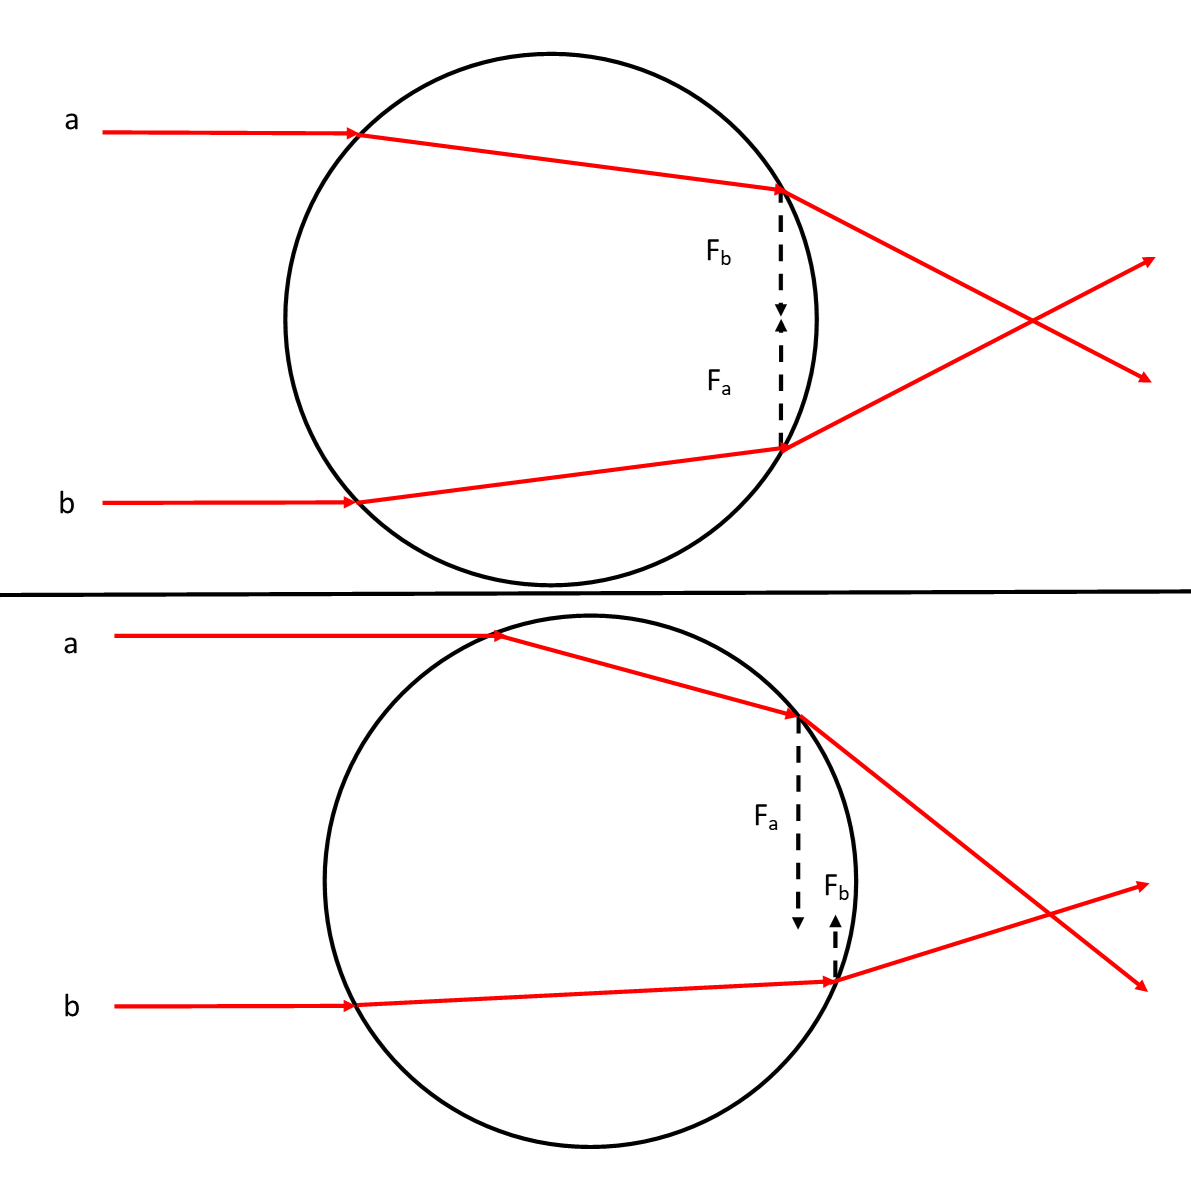
\includegraphics[width=0.65\linewidth]{figs/ot_working_principal.png}
	\caption{Working principle for an optical trap, upper image shows a sphere at the centre of a trap experiences equal forces directed towards inwards. Lower image shows that when displaced 'ray a' is refracted far more than 'ray b' resulting in a net force back towards the centre.}
\end{figure}

\section{Electromagnetism and optical tweezing}
Proper understanding of optical tweezing requires an understanding of how the trapped particle interacts with the trapping laser. From a electromagnetism perspective the laser creates a spatially and temporally coherent electric field that scatters light off of a trapped particle. The laws governing electric and magnetic fields are summarised most succinctly via the Maxwell equations. The differential forms of which are given below:
\begin{align}
    &\nabla \cdot \bold{E} = \frac{\rho_ v}{\epsilon_0} \\
    &\nabla \cdot \bold{B} = 0 \\
    &\nabla \times \bold{E}  = \frac{\delta \bold{B}}{\delta t} \\
    &\nabla \times \bold{B} = j_0 +\frac{\delta \bold{E}}{\delta t}    
\end{align}
These 4 equations describe how the electric and magnetic fields must behave and are also related to one another, any discussion of optical trapping is underpinned by the fact that in all cases the Maxwell Equations must be satisfied. 

The force exerted by an optical tweezer can be subdivided into the gradient and scattering components, for most modelling research this is how the force fields are reported. The gradient force is a conservative force brought about by the polarisation of dielectric materials, anything around 10\% of the trapping wavelength will be attracted along the gradient of the electric field to the region of greatest intensity (for a simple Gaussian Beam this would be at the focal point). The scattering force arises from the scattered field of the trapping beam pushing the target object away from the focal point; unlike the gradient force, the scattering force is non-conservative and is loosely proportional to the particle's Brownian motion. The equilibrium position (where the mean squared displacement is minimised) is found when the gradient force far exceeds the scattering force, interpreting and calculating these forces is dependent on the ratio between the particle size and the trapping wavelength.

\subsection{Ray-Optics Regime}
The Ray-Optics model is the simplest to understand, the theory models the laser as a collection of individual 'rays' that propagate and are refracted according to Snell's Law. Based on the change in direction momentum is transferred to the target particle; with rays closest to the centre of the beam having greater intensity than those rays at the very edge of the beam. Consider a particle struck by two rays in a Gaussian beam (see Fig below), one coming close to the centre, and the other ray coming from the edge. As each ray is refracted by the target sphere a force is imparted onto it, the total force imparted is given by:

\begin{align}
	F_i = Q_i\frac{\Delta n P_i}{c}
\end{align}

Where $Q_i$ is the trapping efficiency, $\Delta n$ is the difference in refractive indices between the solution and the target particle, and $P_i$ is the power of the individual ray. For a beam with a Gaussian intensity distribution $P_i$ will fall off as you move from the centre of the beam. The ray optics model is ideal for  

\subsection{Lornez-Mie Theory}
The Lorenz Mie theory provides an exact solution to the maxwell equations for the scattering caused by an isotropic sphere. The theory describes the scattered wave given off by a dielectric sphere when incident by a plane wave as a summation of partial spherical waves. For any spherical wave the vector fields must solve the Helmholtz wave equation given by:
\begin{align}
	\nabla^2\boldsymbol{E} +k^2\boldsymbol{E} = 0
\end{align} 
This combined with the constraints of Maxwell's Equations leaves very few exact solutions apart from spherical or planar waves, both of which can be converted between with relative ease. For example, a plane wave electric field can be expanded into spherical harmonics and likewise any spherical wave can be described as combination of plane waves offset from one another. For a single plane wave the incident, internal, and scattered fields are given as:

\begin{align}
	E_{inc}(r) &= E_0 \sum_{n=1}^\infty a_{n}M_{1n}^{(1)}(r)+b_{n}N_{1n}^{(1)}(r) \\
	E_{int}(r) &= E_0 \sum_{n=1}^\infty i^n\frac{2n+1}{n(n+1)}\left(-id_{n}N_{1n}^{(1)}(r)+c_{n}M_{1n}^{(1)}(r)\right) \\
	E_{scat}(r) &= E_0 \sum_{n=1}^\infty  i^n\frac{2n+1}{n(n+1)}\left(-ip_{n}N_{1n}^{(3)}(r)+q_{n}M_{1n}^{(3)}(r)\right)
\end{align}

Where $a_n$, $b_n$, $c_n$, $d_n$, $p_n$, and $q_n$ are the expansion coefficients of each of the fields, for the incident field computing its expansion coefficients is possible via analytical methods and are completely dependent on the beam conditions imposed by the user. However, computing the expansion coefficients of the internal and external fields be far more tedious depending on the shape of the target and what properties of the scattered field are desired - all of which is discussed later on. From an optical trapping perspective the force exerted by a focused electric field can be found by computing the maxwell stress tensor which only requires the total magnitude of the incident and scattered fields, essentially computing the momentum contained in the incident beam and how much of it has been transferred to the target particle. 

Lornez-Mie theory can be applied to describe the scattering from any particle regardless of size, however as we either increase or decrease the size of the target particles the infinite series converges allowing one to ignore much of the tedium of Lorenz-Mie theory. The ray optics model is what is achieved when the size of the target particle far exceeds that of the laser wavelength and thus individual ray's can have independent contributions. In the latter case we can simplify the scattering problem by approximating our target as a single dipole, focusing only its interactions with the incident field.

\subsection{Rayleigh Regime}
The Rayleigh approximation is the limiting approximation for describing a particles motion in an electromagnetic field who's wavelength is several times greater than the particle's size. The underlying theory is that a dielectric sphere can be treated as a dipole while in the presence of the electromagnetic field; in which case the scattering force is given simply by the scattering of the induced dipole, and the gradient force is due to the Lorentz force \cite{Gordon1973}. The gradient forces in the principle Cartesian axis are described by Harada et al \cite{YasuhiroHarada1996} in MKS units as a restorative rectangular force field:

\begin{align}
    F_{grad,x} &=-\hat{x} \frac{2\pi n_2 a^3}{c}
    \left(\frac{m^2-1}{m^2+2}\right) \frac{4\tilde{x}/w_0}{1+(2\tilde{z})^2} \times I(r) \\
     F_{grad,y} &=-\hat{y} \frac{2\pi n_2 a^3}{c}
    \left(\frac{m^2-1}{m^2+2}\right) \frac{4\tilde{y}/w_0}{1+(2\tilde{z})^2} \times I(r) \\
    F_{grad,z} &=-\hat{z} \frac{2\pi n_2 a^3}{c}
    \left(\frac{m^2-1}{m^2+2}\right) \frac{4\tilde{y}/w_0}{1+(2\tilde{z})^2} \nonumber \times I(r) \\ 
    & \times \left[1-\frac{2(\tilde{x}^2+\tilde{y}^2)}{1+(2\tilde{z})^2} \right] \\
    \text{where:} \nonumber \\
    I(r) &= \left(\frac{2P}{\pi w_0^2}\right) \frac{1}{1+(2\tilde{z}^2)} 
    exp \left[ - \frac{2(\tilde{x}^2+\tilde{y}^2)}{1+(2\tilde{z})^2} \right]
\end{align}

Where $m$ is the relative refractive index ($n_1/n_2$), $\omega_0$ is the beam waist, and $a$ is the radius of the particle. Scattering force however is dependent on the effective scattering cross sectional area. 

\begin{align}
    F_{scat} &= \hat{z} \left(\frac{n_2}{2}\right) C_{pr} I(r) \\
    \text{where:} \nonumber \\
    C_{pr} &= \frac{8}{3} \pi (ka)^4 a^2 \left(\frac{m^2-1}{m^2+2}\right)^2
\end{align}

The Rayleigh regime allows for easy computation of the gradient and scattering forces due to the assumption that the particle is a point dipole, so much so that higher order scattering problems can be simplified by subdividing the particle into discrete dipoles (see Sec \ref{sec:scattering}). However as the target particle gets larger this assumption fails to accurately describe the trapping force due to the complexity in the gradient field. For particle sizes close to the laser wavelength the scattered field is best described by Lorenz-Mie theory. 

The T matrix method was first developed by Peter Waterman with his 
research into acoustic wave scattering, this would later be extended to 
electromagnetic waves. Put simply, the method sets a boundary condition 
where the incident field within the interior field is cancelled out via 
interference; these boundary conditions allows us to solve the Maxwell 
equations by expanding the incident and scattered fields using spherical 
vector waves. Because the boundary condition ensures that the incident field is halted at the interior surface of the object, the scattering field can be related to the incident field by the objects T-Matrix:

\begin{align}
    \begin{pmatrix}
    q_{mn} \\
    p_{mn} 
    \end{pmatrix}
    = \bold{T} 
    \begin{pmatrix}
        a_{mn} \\
        b_{mn}
    \end{pmatrix}
    = \begin{pmatrix}
        T_{11} \ T_{12} \\
        T_{21} \ T_{22}
    \end{pmatrix}
    \begin{pmatrix}
        a_{mn} \\
        b_{mn}
    \end{pmatrix}
\end{align}

The T-matrix method is exceptionally useful for computing the scattering from any arbitrary shaped particle. However, the T-matrix method by itself can be limited by computation power for aggregates of particles; while possible to compute the scattering of each individual particle the system of equations cannot be solved analytically and must be solved numerically to determine properties for the aggregate for one particular orientation. 

\section{Langevin Equation}
Describing any microscopic motion requires an understanding of a molecules diffusive behaviour, for the case of optical tweezers the most complete model of diffusion is the Langevin equation. Models such as the Fickian, and Einstein derivations are sufficient for macroscopic behaviours the Langevin equation better describes the microscopic characteristics of any diffusive behaviour. The Fickian model is not suitable for the applications of optical tweezers as it assumes that all diffusive motion is driven by a gradient of molecular density, not only is this often not the case but it fails to describe the motion of any single molecule, only the collective behaviour. Einstein's model however considers the collisions experienced by individual molecules, if we assume that all collisions are random and only consider the behaviour after a finite time step $\delta t$ then the individual collisions should cancel out. This is insufficient for our interests as an optical tweezers relaxation time (given by $\tau = \kappa/\gamma$) is often so short that we must consider the individual collisions experienced by any one molecule. The Langevin model of diffusion therefore assumes that the net force on a particular particle is described fully by these individual collisions:
\begin{align}
	m\frac{dv}{dt} + \gamma_0 v + F(t) = W(t)
\end{align}
Where the first term accounts for inertial forces, the second term accounts for friction forces which counteract the particles current motion ($\gamma_0$ is the friction coefficient), and the final term accounts for the random Brownian force. The $F(t)$ is there for convention which accounts for any external forces acting on the particle. We can say that the noise term $W(t)$ has a Gaussian probability, with a correlation function of:

\begin{align}
	&W(t) = \sqrt{2k_BT\gamma_0}\eta(t) \\
	&\langle W_i(t)W_j(t')\rangle = 2k_BT\gamma_0\delta(t-t')
\end{align}

The Langevin model can be extrapolated to describe the diffusive behaviour of an overall system, but for this project we can instead consider the behaviour of some particle with a diffusion tensor $D$ suspended in a viscous fluid and spacially localised by an optical potential with trap strength $\kappa$. Assuming the only external force acting on our particle is the laser the net force should be exactly equal to force of the stochastic collisions due to the fluids thermal energy. If we focus our analysis when the particle is stably trapped and assume that the trap is harmonic we can model the trapping force as a Hookean spring ($F(t) \approx \kappa x(t)$). The full Langevin equation for an optically trapped particle is therefore given as:
\begin{align}
	\label{eq:langevin}
	m\frac{\delta^2x(t)}{\delta t^2} + \gamma_0 \frac{\delta x(t)}{\delta t} + \kappa_x x(t) = \sqrt{2k_BT}\eta(t)
\end{align}

Eq.~\ref{eq:langevin} provides an accurate description of strongly trapped particles, however the analytical solution of the Langevin equation requires integration of the white noise term making it difficult to simulate the trajectory of a given particle \cite{Volpe2013}. Instead it is often far easier to solve the equation numerically and apply use the analytical solution to calibrate and extract information about the particle and fluid, and how the two interact with the optical trap.

\subsection{Finite Difference}
The Finite Difference approach involves discretizing the time and spatial elements in order to approximate the higher order terms. If we assume that $x(t)$ is differentiable to n (we can find its $n^{th}$ derivative) then we can use the Taylor series expansion to get:
\begin{align}
	x(t+\Delta t) = x(t)+\frac{x'(t)}{1!}\Delta t + \frac{x^2(t)}{2!}\Delta t^2+...+\frac{x^n(t)}{n!}\Delta t^n+R_n(x(t))	
\end{align}
Where $R_n(x(t))$ is the remainder term between the Taylor expansion to term n and the actual expression. If we limit our approach to the first derivative only we find that for sufficiently small values of $R_1$ the velocity and acceleration can be approximated as:
\begin{align}
	x'(t) &= \frac{x(t+\Delta t)-x(t)}{\Delta t}=\frac{dx(t))}{dt} \\
	x^2(t) &= \frac{x'(t+\Delta t)-x'(t)}{\Delta t} = \frac{x(t)-2x(t+\Delta t)+x(t+2\Delta t)}{\Delta t^2}
\end{align}
By reversing the time step (i.e. use $-\Delta t$) to approximate the velocity and acceleration based on the previous time steps we can discretize the position by taking finitely small  time steps (i.e. $x(t) = x_i,\ x(t-\Delta t) = x_{i-1}$). The same cannot be done for white noise as no information is known about $W(t)$ at any time. We can instead say that the velocity of a Brownian particle should approximate our white noise as a random walk, where at each new time step the position changes randomly within a given range. Constricting the variance to $\sqrt{2D}/\Delta t$ allows us to represent the white noise using the finite-difference approach as:
\begin{align}
	m\frac{x_i-2x_{i-1}+x_{i-2}}{\Delta t^2} = -\gamma\frac{x_i-x_{i-1}}{\Delta t}+\sqrt{2k_BT\gamma}\frac{w_i}{\sqrt{\Delta t}}
\end{align}
Where $w_i$ is a random real number between -1 and 1, we can say that it is normally distributed around 0 for simulation purposes. We can rearrange this for $x_i$ to approximate the Brownian motion of a particle (setting $x_0=0$), where the characteristic time is $\tau = m/\gamma$. Now in the case of an optical trap the restoration time scale is given by $\tau_{OT}=\kappa_x/\gamma$ which for strongly trapped particles is far greater than the characteristic time, therefore for simulation purposes we can neglect the particle's inertia which allows us to write the motion of an optically trapped particle as:
\begin{align}
	\label{eq:sim_langevin}
	x_i = x_{i-1} + \tau_{OT}\ x_{i-1}\Delta t + \sqrt{2D\Delta t}\ w_i
\end{align} 

This result can be generalised for a 3-dimensional description of an optically trapped particle, where each Cartesian direction has its own unique characteristic restoration time. We see from the result that trajectory is dependent on only a handful of factors, the trap stiffness $\kappa_x$, the fluid viscosity $\gamma$, and the thermal energy of the system $k_BT$ - with the latter two being related by Einstein's formulation of the diffusion coefficient $D = k_BT/\gamma$. Therefore by calculating these parameters to a high degree of precision allows one to get precise description of the forces experienced by a target particle, which in the past has been used for highly accurate force transduction \cite{BergSoerensen2004, Smith2003}.

\section{Calibration Techniques}
\label{sec:calibration_techniques}
There are several approaches for calibrating and characterizing the optical trap, each approach has its drawbacks and benefits so each option should be chosen based on what elements want to be characterized. The basis for each of these methods stems from the analytical solution of the Langevin equation:
\begin{align}
	\label{eq:anylitical_lang}
	x(t) = x(0)e^{-t/\tau_{OT}}+\sqrt{2D}\int^t_0dsW_x(s)e^{-(t-s)/\tau_{OT}}
\end{align}

\subsection{Potential Well Analysis}
The Langevin equation for an optically trapped assumes that the trap acts similar to a Hookean spring that creates a potential well about its center. Therefore a simple analysis method is to understand the height and width of said potential well. 

Potential analysis is a useful technique for estimating the strength of an optical trap; this method assumes that the force acting on the particle is purely conservative, an accurate presupposition if we ignore the motion of the particle as it enters the trap. This is because the scattering force is far more significant far away from the potential well and is negligible if the trap strength is much greater than the thermal fluctuations. With this in mind we can write the probability of finding the particle at position $x$ as:
\begin{align}
	\frac{\rho(x)}{\rho_0} = e^{-\frac{U(x)}{k_{\small{B}}T}} 
\end{align}
which therefore means we can write the potential well as:
\begin{align}
	\label{eq:potential_well}
	U(x)=-k_BT\ ln\left(\frac{\rho(x)}{\rho_0} \right)
\end{align}
Now assuming our laser acts as a Gaussian beam we should be able to describe the probability distribution $\rho(x)$ centred at some equilibrium position $x_0$:
\begin{align}
	\label{eq:prob_dist}
	\rho(x)= \sqrt{\frac{\kappa_x}{2\pi k_BT}}exp\left(-\frac{\kappa_x}{2k_BT}(x-x_{eq})^2\right)
\end{align}
By inserting eq.~\ref{eq:prob_dist} into eq.~\ref{eq:potential_well} we can fit the potential well in order to determine the trap strength $\kappa_x$, and an estimation of the equilibrium position $x_{eq}$. This has some limitations in that the large fluctuations can throw off the fit meaning a longer acquisition time is necessary to properly fit the potential well, making it difficult to characterise weakly trapped particles who may not remain trapped for long. It also provides no information on the particle itself (i.e. the friction coefficient $\gamma$ and diffusion coefficient $D$).

\subsection{Equipartition method}
The Equipartition method is by far the fastest and simplest means for estimating the trap strength but unlike Potential Analysis is limited strictly to harmonic potentials. This can be often not the case for highly focused beams, as the trap strength can vary due to polarisation differences. Simply put we can use the equipartition theorem to relate the potential well to the particle's thermal energy using eq.~\ref{eq:prob_dist}:
\begin{align}
	\left<U(x)\right> = \frac{1}{2}\kappa\left<(x-x_{eq})^2\right> &= \int_{-\infty}^{\infty}\rho(x)(x-x_{eq})^2 = \frac{1}{2}k_BT \\
	\implies \kappa_x &= \frac{k_BT}{\left<(x-x_{eq})^2\right>} 
\end{align}

By taking a time average over multiple trajectories to get $\left<x-x_{eq}\right>$ we can get a fairly accurate estimation of the trap strength. Because of this requires a time average of the particle's displacement any large errors in the position measurement can have knock-on effects. Likewise with the potential-analysis route, no information is gleaned about the particle itself.

\subsection{Mean Square Displacement}
Mean square displacement (MSD) is a common means of describing the random motion of a given particle (or group of particles). This is useful information if say for example we want to understand reaction kinetics on the surface of a catalyst, if we know how far its likely to move from the surface we can tell if its likely to react when a catalytic site becomes available. As it pertains to colloids, consider a suspension of silica spheres immersed in a fluid undergoing Brownian motion (as described by the Langevin Equation) so that:
\begin{align}
	mx''(t) + \gamma x'(t) = \eta(t)
\end{align}
Where $\eta(t)$ is a random white noise variable that is directly related to the thermal energy of the surrounding fluid. If the motion is truly random then we should see an average displacement of 0 regardless of how long we measure for. If we wish to understand the effects of a given external factor (i.e. an electric field or localised heating), simply looking at displacement will reveal nothing of value as its difficult to differentiate between diffusive and a biased motion. 

For each sphere we can record its position in the $x-y$ plane and measure its displacement from a set reference point; for example with an optical tweezer this could be the beam focus. We can measure the MSD by forming a 'window' between two points in time of the trajectory (i.e. $t \&  t+\tau$) and sliding this window along the entire trajectory length - to eliminate -ve displacements we take the square - we can then take the average of this series. Repeating over a range of time lags allows us to describe the MSD as a function of $\tau$:
\begin{align}
	MSD(\tau) = \left<|x(t+\tau) - x(t)|^2\right>
\end{align}

If we use eq.~\ref{eq:anylitical_lang} for an optical tweezer we can expand out the squared term to get an analytical expression for the MSD as a function of time lags:
\begin{align}
	\label{eq:MSD}
	MSD(\tau) = \left<|x(t+\tau)^2-2x(t+\tau)x(t)+x(t)^2|\right> = \frac{2k_BT}{\kappa_x}\left[1-e^{-\frac{\tau}{\tau_{OT}}}\right]
\end{align}
From this expression its evident that the mean squared displacement increases with larger values of $\tau$ until it reaches a maximum value as shown below by the dotted line.
\begin{figure}
	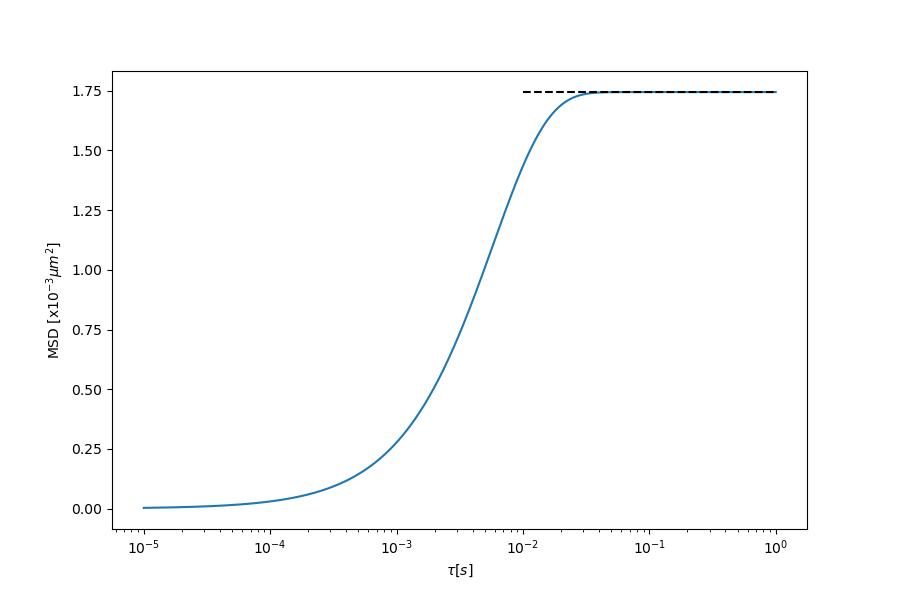
\includegraphics[width=0.67\linewidth]{figs/MSD.png}
	\caption{Example mean squared displacement using eq.~\ref{eq:MSD}, for a $1\mu m$ sphere trapped by an optical potential well. The dotted line represents the upper limit of the sphere's displacement due to the optical trap.}
\end{figure}
The MSD plot can be subdivided into two regimes, when $\tau \gg \tau_{OT}$ the particle is experiencing the harmonic potential described by the equipartition theorem, and when $\tau \ll \tau{OT}$ the particle is said to be freely diffusing within the trap focus. Of course for a freely diffusing object the MSD will never reach a plateau value, comparing MSD's for different particles provides a simple visual indicator of the difference in trapping strength. The MSD method is an already very versatile analytical tool for diffusive motion, however it is rather slow in computing time meaning it is only really beneficial when a high degree of accuracy is required and shorter time resolutions are unavailable - such as using a quadrant photo diode instead or a high speed CCD.

\subsubsection{Angular Mean Square Displacement (MSAD)}
It is also possible to plot the angular MSD (MSAD) using simulative data, however there is yet to be a analytical expression for the MSAD of a freely diffusing particle. Vigilante \textit{et al} \cite{Vigilante2020} derived the upper limit of a dimer's MSAD along its long axis by assuming it was strongly trapped and so had limited angular motion, there expression gives:
\begin{align}
	\lim_{\tau\to\infty}\left<(\Delta u_z)^2\right> = 
	2\left[1-\frac{1}{4\beta\kappa_r} 
	\left(\frac{exp(\beta\kappa_r)-1}
	{exp(\beta\kappa_r)F(\sqrt{\beta\kappa_r})
	}\right)^2\right]
\end{align}  
Vigilante's paper expressed that they couldn't compute $MSD(\tau)$ because they couldn't solve the Einstein-Smoluchowski equation which describes the diffusion constant for dielectric particles. This would require a full description of a particle's electrical mobility and charge distribution - the latter could be achieved via a discrete dipole approximation, the former would be dependent on both the particle's position but relative orientation to the electric field.

\subsection{Power Spectrum Density (PSD)}
The power spectral density (PSD) method is by far the most versatile method for observing the dynamics of any object within an optical trap, allowing for fast calibration times while also quickly filtering out typical noise sources. Taking the Fourier transform of a particle's trajectory yields:
\begin{align}
	\hat{x}(f) = \frac{(2D)^{1/2}\hat{\eta}}{2\pi(f_c-if)}
\end{align}
where $\hat{\eta}$ is the Fourier transform of the white noise, where the values are exponentially distributed as opposed to being normally distributed in the time domain \cite{BergSoerensen2004}, the correlation function is given as:
\begin{align}
	\left<\hat{\eta_k}\hat{\eta_l^*}\right> = t_{msr} \delta_{k,l} \rightarrow \left< \eta^4 \right> = 2t_{msr}
\end{align} 
We can therefore ignore the white noise from our analysis by looking at the spectral density of $\hat{x}(f)$: 
\begin{align}
	S_x = \frac{\hat{x}^2}{t_{msr}} = \frac{D}{2\pi(f_c^2+f^2)}
\end{align}

We can fit the Lorentzian via a simplified geometric series $S_x = 1/(A+Bf_k^2)$ which allows us to compute both the diffusion coefficient (in arbitrary units) and the corner frequency $f_c$ which is directly related to the trap strength via $f_c = \kappa_x/(2\pi\gamma)$. Like with the analytical expression of the mean squared displacement we see two distinct regions, when $f\ll f_c$ the PSD reaches a plateau value that when converted to length units represents the maximum displacement the particle can move beyond the focus, however when $f\gg f_c$ the PSD falls off exponentially which denotes the particle is freely diffusing within the beam focus.
  
The Lorentzian relationship is only valid for frequency terms up to the Nyquist frequency (half of our sampling rate), this is because we are only taking a finite sampling of the particle's trajectory meaning the signal is aliased. Berg and Sorensen provide a suitable modified Lorentzian to account for the aliasing effects \cite{BergSoerensen2004}:
\begin{align}
	S_x = \frac{(\Delta x)^2\Delta t}{1+c^2-2c\cos{2\pi f_k\Delta t/N}}
\end{align}
Where N is the total number of samples taken, $\Delta x \ \& \ c$  have no direct physical interpretation and are defined in \cite{BergSoerensen2004}. Further modifications can be made to the power spectrum model but this is only useful when a high degree of accuracy is necessary. Typically power spectra are recorded using a Quadrant Photo Diode (QPD), which records motion in voltage units, not in units of length. To convert between the two we have a few methods: Firstly if we have a mono-disperse suspension of particles, the laser can be scanned across the surface of our target particle; so long as the particle's size is known a linear conversion factor can be used to convert from voltage to length units. Secondly, if the size distribution is very wide but each particle can be accurately sized, then a conversion factor can be approximated by comparing the fitted value of the diffusion coefficient, and the reported value given by the Stokes-Einstein relation.

\begin{align}
	D_{SE} = \frac{k_BT}{\gamma_0} \Rightarrow Conversion\ Factor \ [m/V]= \sqrt{\frac{D_{SE}}{D_{fit}}}
\end{align}

With the latter method, the local fluid viscosity must be known to a high degree of accuracy, depending on the local heating effect this may be as trivial increase or it may be significant enough to drastically alter the characterisation. PSD analysis is often seen as the gold standard for calibration as it can be fine tuned to the point that optical forces can be computed on the order of $10^{-15} N$ \cite{BergSoerensen2004}, it captures all of the information acquired by other calibration techniques while filtering out noise and requiring a relatively small amount of data collected. 


\chapter{Effects of localised shearing on crystal growth and nucleation}
As outlined in Chapter 1, the original outline of the PhD was to investigate the possibility of using optical tweezing as a means of initiating and controlling nucleation by generating fluid flow within a small droplet of supersaturated solution. The goal of which would be to allow the understand the influence of shearing on nucleation at a micro level as compared to larger scale results. It has been shown that for macro-scale systems, the likelihood of nucleation increases to a maximum value under increased shearing \cite{Debuysschere2023, Mura2016}. Theoretical research into the matter identified two competing effects that effect a crystal in moving fluid fields; firstly, nucleation is enhanced due to the increased mass transfer of solute material; and secondly, shear flow against the crystal surface leading to a decrease in growth \cite{Mura2016}. These two competing effects are validated by experimental work using glycine solutions, showing that beyond a certain shear rate the nucleation rate is reduced \cite{Debuysschere2023}. 

\section{Optical Tweezer Equipment}
In general, all optical tweezers require a low power laser driver, two microscope objectives (one for trapping and one for imaging), a means of controlling the position of the loaded sample, and a means of isolating vibration signals. The laser used for this project was a 1064 nm near infrared laser - provided by CNI Lasers – that has an adjustable power supply to vary the energy output of the laser. Experimental work has shown that the trapping efficiency increases with beam diameter up until it exceeds $\frac{2}{3}D_{obj}$ where $D_{obj}$ is the diameter of the objective aperture. To expand the beam front we utilise a Galilean beam expansion arrangement (indicated by $L_1$, and $L_2$) as recommended for high power laser applications. In our initial experiments the beam expansion provides a $4\times$ magnification; however, in later experiments where we utilise a galvano-mirror the beam expansion is $3\times$ and then the 4f correlator provides a further $1.25\times$ magnification. Afterwards the laser is passed through a dichroic mirror that reflects oncoming infrared light but allows the passage of LED light through, this is to prevent the laser from interfering with the CCD imaging. By increasing the numerical aperture of the objective, the gradient force at the focal point is increased; the trade-off being that the for higher NA values the trapping depth is reduced due to spherical aberrations. While it is possible to increase the trapping depth by adjusting the objective's tube length this approach is incompatible with our trapping arrangement. The condenser objective refocuses the scattered laser light and also provide an aperture for an imaging LED to illuminate the focal plane. Samples are loaded onto a piezo driven table to that is inserted between the trapping and condensing objectives; the piezo drivers allow for sub-micron control of the sample position to a degree as small as a 10 nm. To detect and monitor the position of a trapped particle a quadrant photo diode (QPD) was utilised. 

\subsection{Position detection methods}
There are several methods for monitoring the position of 
A QPD is a typical example of a position detection system commonly used 
in optical tweezers due to their high sampling rate, high degree of 
precision, and ease of set up. The QPD is constructed of four photo 
diodes assembled in a quadrant formation, when a particle is trapped the 
interference pattern produced is directed onto the QPD, with the maximum 
intensity mapping to the particle's centre of mass. By summing the 
horizontal and vertical quadrants together the particle's centre of mass 
is tracked in the x-y plane. While the tracking is accurate the QPD 
needs to be calibrated in order to convert the voltage signals into 
actual distance reading. 


\section{Synthesis of Birefringent Micro spheres}
\label{sec:vaterite}
Generation of fluid shear can be achieved via two avenues: Firstly, by 
utilising circularly polarised light it is possible to transfer angular 
momentum from the laser to the trapped entity. Secondly, one can 
directly move the trap within the imaging plane by steering the beam 
using either a galvanometric mirror or gimbal mirror. The following 
chapter outlines the work done with shear generated by circularly 
polarised light and the challenges of applying this to localising 
nucleation. 

There are several options for particles that can be rotated using 
optical tweezers []. Over the course of this project two different micro 
spheres where investigated, vaterite and liquid crystal droplets. Both 
can be readily synthesised in the lab and are will rotate at a variety 
of sizes. While silver nano particles were considered their high cost 
and small size meant they were disregarded as an option for optical 
rotation. 

\subsection{Rotation of Vaterite micro spheres}
Vaterite is a polymorph of calcium carbonate that is rarely seen in 
nature due to its low stability. However unlike its other polymorphs of 
calcite and aragonite, when synthesised vaterite will typically form 
small spherical particles making them ideal for optical trapping. 
Synthesis of vaterite micro spheres requires fine control of the nucleation process in order to maintain polymorphic control. 
	

\chapter{Complex Langevin dynamics of simple spherical aggregates}
Much of the theory discussed in Chapter 2 assumes that the target particle in question will be a single sphere, one who's scattering and motion is easily generalised. However, while working with dense colloidal suspensions, one often ends up trapping more than one microbead. Li and Arlt \cite{Li2008} studied the case of two microspheres trapped in a single OT and found that multiple trapped beads could be mistaken for a single trapped bead with altered trap stiffness. Theoretical studies on the case of two trapped microspheres by Xu et.al., \cite{Xu2005} employed a ray-optics based model to show that the two trapped beads are brought into physical contact with each other by optical forces and they also calculated the axial equilibrium positions of the two trapped beads as a function of their size. Experiments in \cite{Praveen2016} confirmed that the two trapped beads indeed experience different trap stiffnesses in the vicinity of the same potential well. There are further discussions looking into the dynamics of a whole host of asymmetrically shaped particles \cite{Loudet2014, ShengHua2005, Chetana2022}, their results all showing that predicting the behaviour an arbitrary shaped particle comes with great difficulty due to the fact that the optical force is dependent on a greater number of variables such as orientation and size factors.

In this chapter we consider how the addition of a second sphere into an optical trap can radically effect its dynamics, to the extent that one can no longer rely on typical calibration techniques to characterise the interactions.

\section{Positional and Orientational dependence of Trapping forces}
If we wanted to start from first principles and determine the trap strength on our target particle the first step would be to locate the harmonic traps relative to the trap focus. The methodology for computing optical forces has been covered extensively for a number of different trapping conditions \cite{RanhaNeves2019}, so it is relatively easy to compute the trapping force and determine where a simple sphere would be located relative to focal point of the laser. We can do so because the optical force is only dependent on the particle's relative position. If we instead consider a asymmetric dimer for example we see just by inverting the particle then a secondary harmonic trap can be found below the focus.

\begin{figure}[h]
	\centering
	\begin{subfigure}{.475\linewidth}
		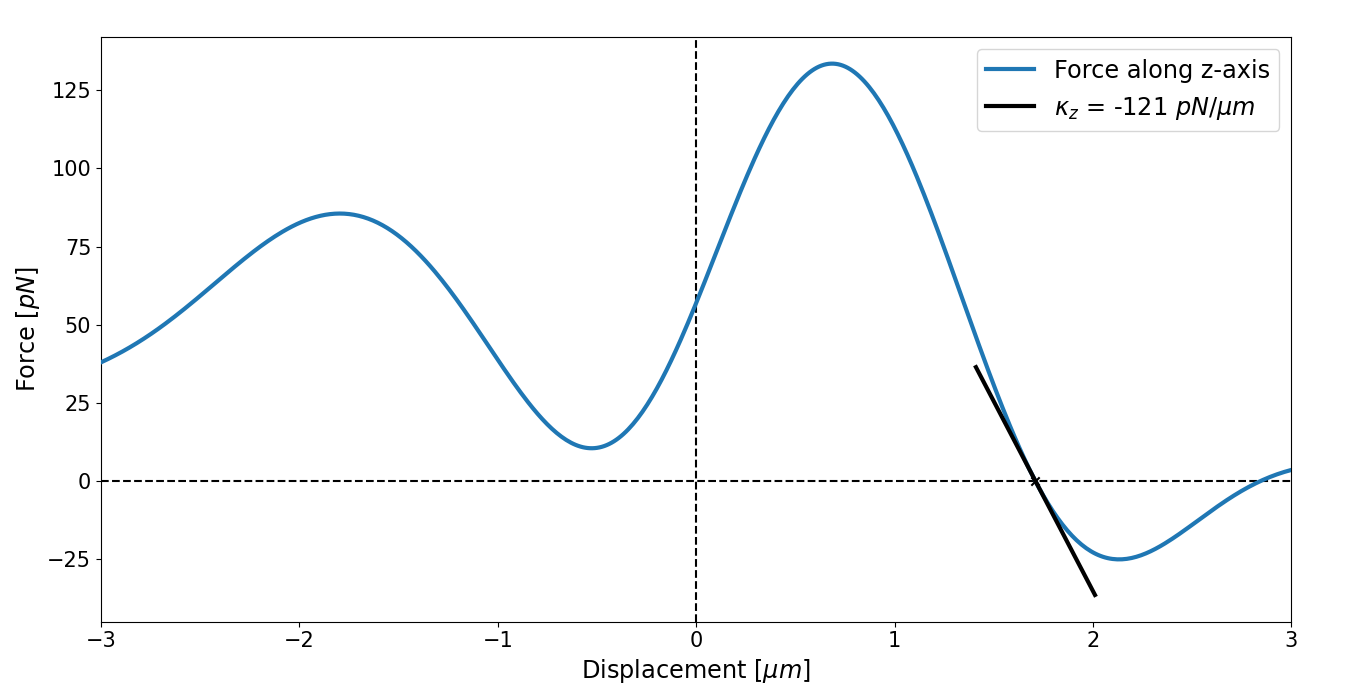
\includegraphics[width=\linewidth]{figs/lam=2_theta=0.png}
		\caption{}
		\label{lam=2}
	\end{subfigure}\hfill % <-- "\hfill"
	\begin{subfigure}{.475\linewidth}
		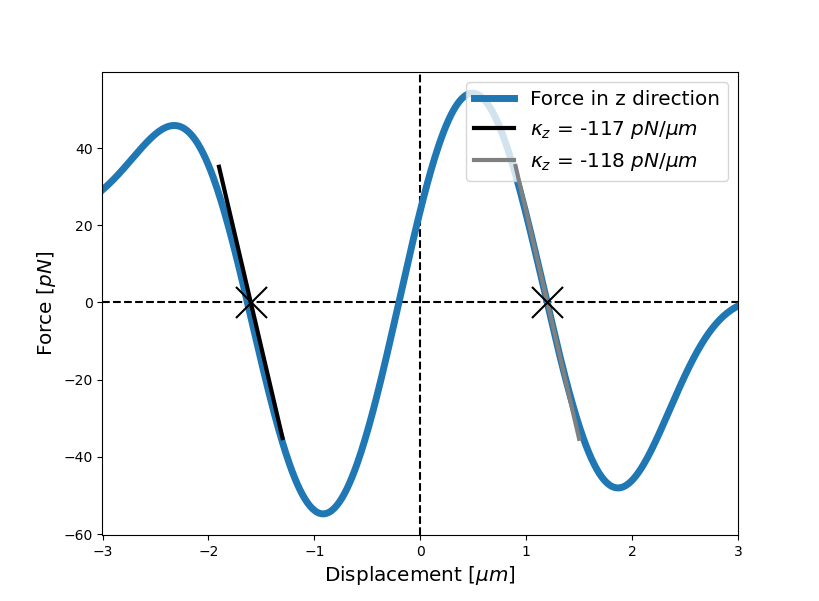
\includegraphics[width=\linewidth]{figs/lam=2_theta=180.png}
		\caption{}
		\label{lam=2_inverted}
	\end{subfigure}\hfill % <-- "\hfill"
	\medskip
	\begin{subfigure}{.475\linewidth}
		\centering
		\raisebox{65pt}[0pt][0pt]{\makebox{}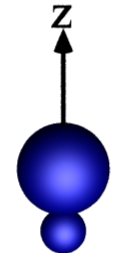
\includegraphics[width=0.3\linewidth, keepaspectratio]{figs/theta=0.png}}
		\label{large over small}
	\end{subfigure}
	\begin{subfigure}{.475\linewidth}
		\centering
		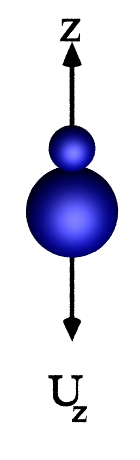
\includegraphics[width=0.3\linewidth, keepaspectratio]{figs/theta=180.png}
		\label{small_over_large}
	\end{subfigure}
	\caption{Plots of force vs displacement of the point of the contact of the spheres (µm) for the case of a dimer of size ratio 2. (a) is the case where the smaller sphere is orientated with the beam propagation direction. (b) is the inverted case, smaller sphere oriented against the propagation direction. Renders to visualise the dimer orientation are shown below each plot The black lines on each force-curve is a linear fit with the slope being reported as the trap stiffness in the legend.}
\end{figure}

We can see that the trap below the focus is comparable in strength to above the focus, however the difference in the transverse strength is far more noticeable. As shown in Fig~\ref{fig:transverse_force}, the dimer's orientation and relative position significantly changes the force curve; not only is the trap wider when inverted but the trap stiffness is increased. This highlights one of the challenges involved with studying asymmetric particles, even though its a simple enough process to trap them they maybe characterised very differently depending on their relative position and orientation towards the trap. This can have a significant impact on rheological studies - or attempting to probe any local property - as the variance in trap strength can result in large errors over repeated measurements. 
\begin{figure}
	\centering
	\label{fig:transverse_force}
	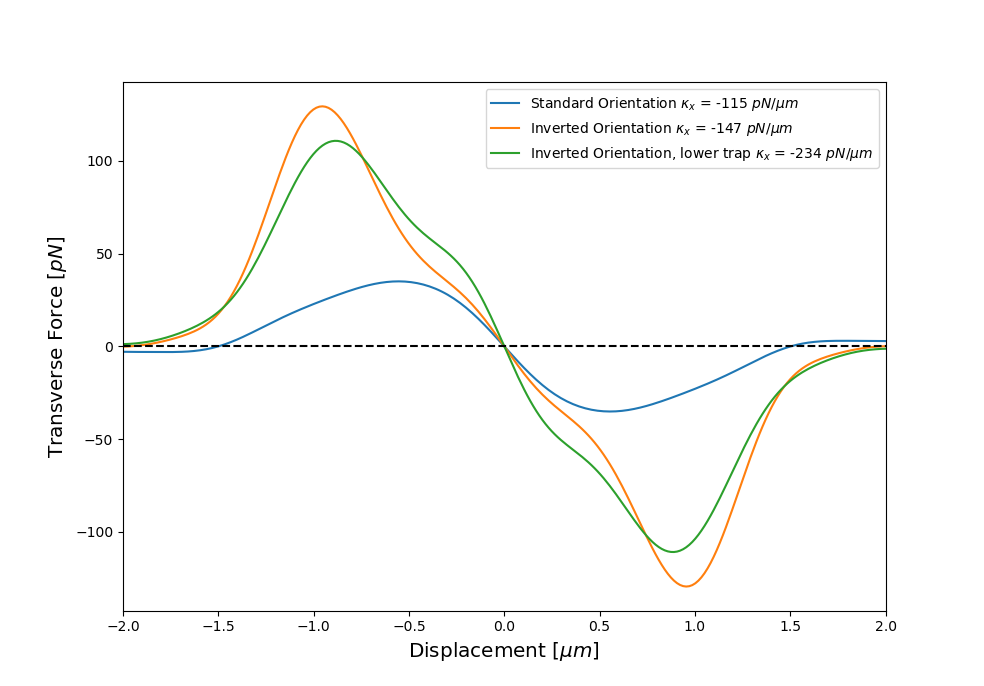
\includegraphics[width=0.67\linewidth]{figs/transverse_force.png}


	\caption{Plots of force vs displacement of the point of the contact of the spheres (µm) for the case of a dimer of size ratio 2 while being displaced in the transverse plane. With the blue curve representing the force response for a dimer in its standard orientation, orange being the inverted case, and green the same case but placed below the focus.}
\end{figure}

For completeness the harmonic traps were located for dimers across a range of size ratios - from $a_1/a_2 = 1$ to $a_1/a_2=10$ - while also recording the trap stiffness for each trap. As $a_2$ decrease the dimer begins to approximate a single homogenous sphere - at least in terms of location and trap strength. However, for intermediate sized dimers (between $a_1/a_2 = 1.1$ to $a_1/a_2=4$), a second harmonic trap appeared below the trapping focus. Previous work using the ray-optics model have confirmed even in the case that two spheres begin separated the electric field will align the molecules as such that they make contact and are trapped together about a single trapping position \cite{Xu2005}. Furthermore it has been shown through proper manipulation of the Gaussian or Bessel beam modes that any number of trapping potentials can be developed \cite{Shahabadi2020}. This result however, is the first example of an orientation dependent trapping situation using only a $TEM_00$ beam. 

\begin{figure}[t]
	\centering
	\begin{subfigure}{0.5\linewidth}
		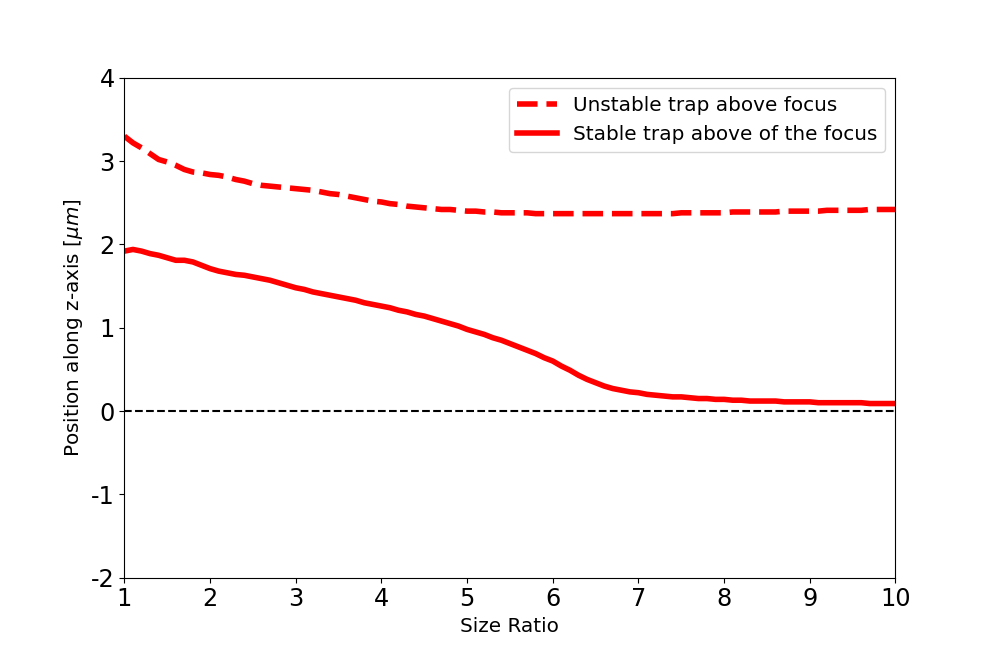
\includegraphics[width=\linewidth]{figs/Equillibrium_positions.png}
		\caption{}
		\label{eq_pos}
	\end{subfigure}\hfill % <-- "\hfill"
\medskip
	\begin{subfigure}{0.5\linewidth}
		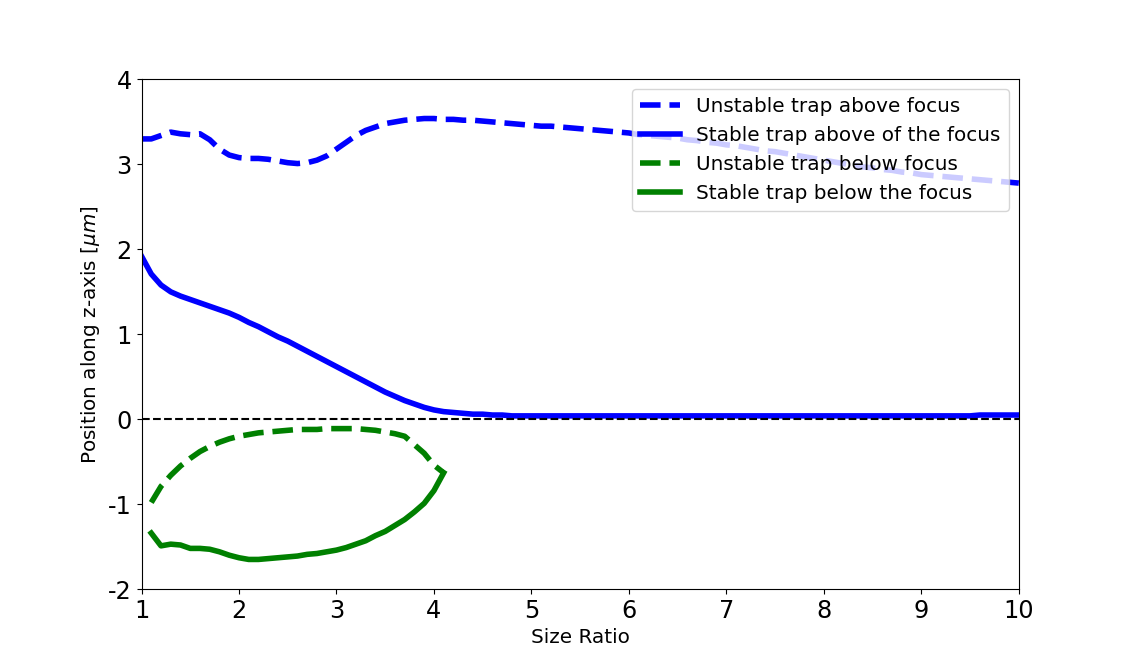
\includegraphics[width=\linewidth]{figs/Equillibrium_positions_inverted.png}
		\caption{}
		\label{eq_pos_inverted}
	\end{subfigure}
	\caption{Equilibrium positions of optically trapped dimers with varying size ratio, dotted lines represent unstable traps whereas solid lines represent stable trapping positions. (a) shows that dimers with their smaller sphere orientated away from the focus have an expected single trapping position. (b) shows that when the same dimer is inverted $180^\circ$ there are now stable traps along the beam axis, one below the focus and one above the focus.}
\end{figure}

This was only seen when the dimer is orientated with the smaller sphere above the larger sphere, when the dimer is flipped then the force curve only intersects the x-axis once, regardless of size ratio. More noteworthy is that in this orientation the dimer’s equilibrium position reaches its limit at a smaller size ratio; before it took a size ratio of 1:4 to achieve a final equilibrium position whereas now the second sphere needed to shrink until it was 1/7th of the first sphere’s size before the equilibrium position settled. This would suggest by having a second sphere behind the first, the momentum transfer from the beam to the dimer is diminished resulting in a weaker force pushing against the dimer as it sits within the trap. And when the dimer is flipped this shielding is lost and so both beads are being pushed by the beam.

Computing the equilibrium positions when a dimer is aligned with the electric field is relatively trivial as the orientational torque is minimised (see Eq.\ref{eq:opt_torque}), meaning once trapped the dimer is unlikely to change orientation enough to escape the trap. However, that does not rule out the possibility that there is a stable orientation that is not strictly vertical, in fact most experimental work with symmetric dimers will trap them lying perpendicular to the beam direction \cite{Ahn2018}. Unlike before where we can simply find the trap by varying the dimer's vertical position its instead more prudent to run a multitude of smaller simulations at a variety of starting positions and orientations. An example for a dimer of size ratio 2 is shown below:

\begin{figure}
	\centering
	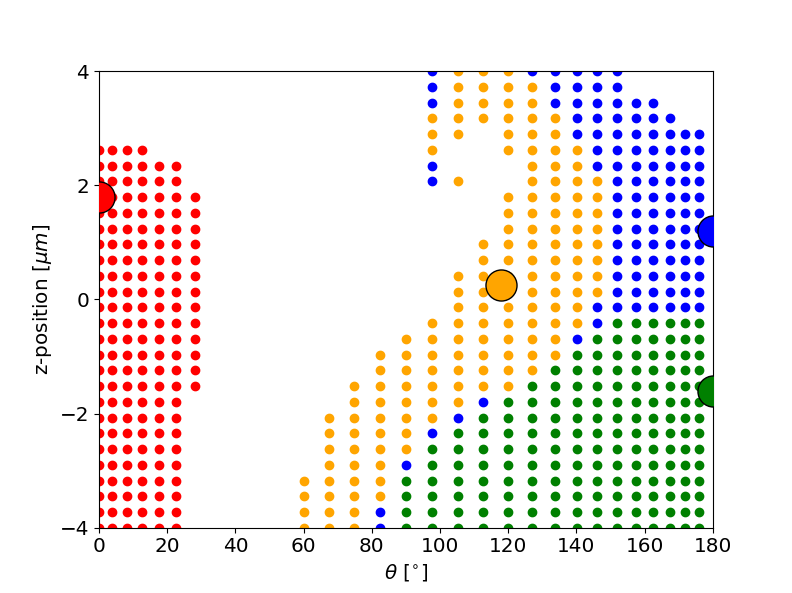
\includegraphics[width=0.75\linewidth]{figs/off_axis_trap.png}
	\caption{Trajectory map of simulations ran using a dimer of size ratio 2 with a laser power of 500 mW. The stable points are indicated by the larger spheres and the starting conditions are colour coded to match the stable point they end up in.}
\end{figure}

Interestingly the trap strength of the these off-axis traps are similar in magnitude to the vertically aligned traps, but when the laser power is lowered (to ~5 mW) the traps become metastable resulting in the dimer escaping from after some random time in the trap. 

\section{Simulative QPD}
A QPD is simply a measure of the total electric field incident on a photo diode, in order to accurately simulate a QPD response careful consideration of how the Electromagnetic fields are defined is required. 

\subsection{Incident beam}
\label{sec:scattering}
The incident beam is simple enough to define given our set up parameters, for the sake of simplicity we assume that our beam is a Laguerre-Gaussian beam of mode $[0.0, 0.0]$ (which is simply a pure Gaussian beam). *Ott* uses a point matching approach to approximate the beam shape coefficients of the incident field by fitting it to the far field estimate, the beam is of the form:

\begin{align}
	E_{inc}(kr)=\sum^\infty_n\sum^n_{m=-n}a_{mn}RgM_{nm}(kr)+b_{nm}RgN_{nm}(kr)
\end{align}

Where $RgM_{nm}(kr)$ \& $RgN_{nm}(kr)$ are regular vector spherical wave functions, *ott* allows us to change the basis of the the incident beam to suit our needs, because we are measuring in the far field we want to set our incident beam to be an outgoing spherical wave so that we can compute the intensity on the QPD. For spherical waves the field can either be expressed as an incoming/outgoing wave (with a singularity at the origin) or as a regular wave around the origin; for incoming/outgoing waves the wave functions use the first/second forms of the Hankel function respectfully. In order to compute the regular spherical wave at the origin we replace the Hankel function with the Bessel function which is simply the average of the first and second forms of the Hankel function, so at the origin we avoid a singularity of the EM field.  

We can if we want further restrict the incident beam by applying setting the truncation angle to match our microscope object, this essentially applies a cut off point to the In order to compute the scattering from the target particle *ott* uses the t-matrix method, this is not essential for a simple sphere but is far more important for complex shaped particles such as our dimers. If the T-matrix is loaded in from *mstm* we need to convert the *mstm* t-matrix to a form more suitable for *ott*:

\begin{align}
	\begin{pmatrix}
		p_{nm}\\
		q_{nm}
	\end{pmatrix} =T 
	\begin{pmatrix}
		a_{nm}\\
		b_{nm}
	\end{pmatrix} = 
	\begin{pmatrix}
		aT^{TM}_{nm} & aT^{TE}_{nm}\\ 
		bT^{TM}_{nm} & bT^{TE}_{nm}
	\end{pmatrix}
	\begin{pmatrix}
		a_{nm}\\
		b_{nm}
	\end{pmatrix}
\end{align} 

For *mstm* the T-matrix is packed as a column vector:

\begin{align}
	T_{MSTM} = 
	\begin{bmatrix} 
		aT^{TE}_{n,-n} & bT^{TE}_{n,-n} \\ 
		aT^{TE}_{n, -n+1} & bT^{TE}_{n, -n+1} \\ 
		... & ...\\ 
		aT^{TE}_{n,n} & bT^{TE}_{n,n} \\ 
		----&----\\ 
		bT^{TM}_{n,-n} &bT^{TM}_{n,-n} 
	\end{bmatrix}
\end{align}

Where as *ott* packs packs the T-matrix with sub matrices:

\begin{align}
	T_{Ott} = 
	\begin{bmatrix} 
		\begin{pmatrix}
			aT^{TM}_{n,-n} & aT^{TE}_{n,-n}\\ 
			bT^{TM}_{n,-n}&bT^{TE}_{n,-n}
		\end{pmatrix} \\ 
		\begin{pmatrix}
			aT^{TM}_{n,-n+1} & aT^{TE}_{n,-n+1}\\ 
			bT^{TM}_{n,-n+1} & bT^{TE}_{n,-n+1}
		\end{pmatrix}\\
		....\\ 
		\begin{pmatrix}
			aT^{TM}_{nm} & aT^{TE}_{nm}\\ 
			bT^{TM}_{nm} & bT^{TE}_{nm}
		\end{pmatrix}
	\end{bmatrix}
\end{align}

\subsection{Scattered and Total Fields}
With the T-matrix in hand we can compute the scattered beam by multiplying our beam shape coefficients with the T-matrix to get out the scattered field. Now in order to simulate a real QPD we need to account for the motion of our target particle within the trap, taking a typical trajectory file we read off each line in order to translate and rotate the beam. Translation is a rather simple process, simply involving us to shift the beam laterally, small deflections are generally unnoticeable for the incident beam but are much more noticeable in the scattered field (the below figure shows the result of shifting the incident beam $1\mu m$ to the right):

The QPD does not just pick up the scattered light however, it instead is receiving a combined signal from both the incident field and scattered field simultaneously, as mentioned by \textcolor{red}{Rohrbach} the total intensity can be computed by taking the magnitude of both the incident field *focused at the origin $[0,0,0]$* and the scattered field originating from $[\delta x, \delta y, \delta z]$ (top left and bottom right plots in the above figure). This means we do not need to worry about any translation effects being 'double-counted' in the QPD's signal as we are only shifting the scattered field meaning the QPD signal is only picking up the interference due to the shifted scattered field. I conducted some unitary tests where I scanned the beam position laterally along the x-axis and measured the QPD's 'x-signal' for x, circular and y-polarized light which yielded the following QPD responses. The target particle was $1.57\ \mu m$ and the scan range is set to $[-4, 4 \mu m]$

Where $S_x$ is given in blue, and $S_y$ is given in orange, the plots make it clear that the polarisation of the beam have a minimal effect on the QPD signals if the particle is traversing in one direction, its clear that the displacement from the beam centre is far more important than the polarization of said beam. This is backed up when we look at \textcolor{red}{Rohrbach's} results, who studied a $150\ nm$ sphere ($n=1.57$) submerged in water with a focusing lens of numerical aperture 1.2, and beam power of $3\ mW$. The condensing lens' numerical aperture was not set to a particular value and was instead varied between 0.13-1.2, as a compromise we selected a condenser numerical aperture of 0.525, corresponding to a acceptance angle of $31.6^\circ$. 

Where the points are Rohrbach's results and the solid line's are our QPD's own replication. The dashed horizontal lines on the left represent the maximum displacement in the lateral displacement which is given by the combined beam radius and particle radius (assuming a beam radius of $0.54\ \mu m$); we can say that any displacements beyond this distance, while non-zero these displacements are unlikely to occur while a particle is trapped at the focus. Whereas the right most plot's dashed horizontal lines represents the Rayleigh range of the Gaussian beam, this represents the transition between plane wave and spherical wave regimes. Interestingly while our results close to Rohrbach's while close to the focus we see it begins to diverge beyond the first peak, this shouldn't be an issue for a typical optical tweezer calibration as we can assume that the maximum displacement will be within this linear regime. 

Now the above plots only consider the QPD response to movements along the cartesian axis, however obviously for any Brownian motion the movements are a combination of displacements in each cartesian direction. We might assume naively that any displacement $\Delta r$ will result in a linear combination of QPD responses; for low precision force measurements this assumption is adequate, however when high precision is required we find that this assumption is longer adequate due to something referred to as cross-talk. Cross talk arises when movement in one direction results in a QPD response change in the other orthogonal direction, there is no one reason for this effect, it could be a result of differing sensitivity in the photo diodes, it could be because the scattering is slightly asymmetric meaning the scattering falls outside the QPD, or it could be a result of mis-alignment in the set up. This can have unintended effects, for example it may lead to the apparent rise of a curved trajectory rather than a straight path: Consider a particle moving purely along the x-axis, with 0 cross-talk the QPD response should perfectly match the above curve $S_x(x,0,z_0)$, with $S_y$ being flat in comparison; if however there is cross talk between the channels then $S_y$ will have some significant non-zero value (or it may even grow with increasing displacement), implying that the particle is actually moving in both the x and y directions simultaneously.  First we checked for this by measuring the QPD response for random positions within the XY plane:

Where $S_x$ is plotted on top and $S_y$ is plotted below, as shown by the above plot we see that they still possess similar shapes to the previous plots but now with additional noise terms, making it clear that for any trajectory there will be cross talk. This means that trying to get a one-to-one measurement of the particle's displacement is not possible by simply looking at the QPD response, to do that we can need to calibrate the trap. 

\textcolor{red}{Berg and Flyvbjerg} have an excellent breakdown for accurately calibrating an optical tweezer, in addition they discuss how to minimise cross-talk effects. For two correlated power spectra, the cross correlation is given as:

\begin{align}
	P_{x} = |\hat{S}_x(f)|^2 \\ 
	P_{y} = |\hat{S}_y(f)|^2 \\
	\rightarrow P_{xy} = Re(\hat{S}_x\hat{S}^*_y)
\end{align}

Now if the two directions are correlated then $|P_{xy}|^2/P_xP_y$  should be non-zero for all frequencies, in order to eliminate cross-talk effects we need to minimise the cross-correlation for all frequencies. They showed that it is possible to find a transformation of the time series $(x(t), y(t))$  to one that possesses the property that $P_{x'y'}(f)=0$ for all frequencies. They found these transformed positions by minimising the sum cross-correlation:

\begin{align}
	\sum\frac{P_{x'y'}}{P_{x'}P_{y'}} = \sum\frac{(1+bc)P_{xy}+cP_x+bP_y}{(P_x+2bP_{xy}+b^2P_y)(Py+2cP_{xy}+c^2P_y)}
\end{align}

Where b and c are fitting parameters, by minimising this function one can adjust each spectra in order to eliminate cross talk effects and provide a more accurate calibration of the optical trap. Furthermore with the fitting completed, the time series can be then transformed in order to eliminate the cross talk effects:

\begin{align}
	x'(t) = S_x(t) + bS_y(t),\ y'(t) = S_y(t) + cS_x(t)
\end{align}

Where $x'$ and $y'$ are now uncoupled coordinates that when Fourier transformed provide the uncorrelated power spectrum. With the fitting complete we can now adjust our time series in order to get a replication of the lateral trajectory. 

\section{Rotations and Asymmetric particles}
Rotational motion is something that is not often necessarily considered when characterising Brownian motion, often because separating the contributions from rotational and translational motion is challenging. Depending on the rotational and translational trap stiffness the collected QPD signal will be aliased and typical calibration techniques cannot characterise the particle and trap interactions. This is often why most of the research into trapping asymmetric objects does not delve into power spectra analysis, as there is no real way of modelling the QPD response from an asymmetric object. 

Now for isotropic scatterers any rotation is often not an issue when it comes to QPD analysis, even if a sphere rotates $180^{\circ}$the scattering should be identical (assuming its relative position is the same). Now *ott* deals with both translations and rotations by moving the beam itself and computing the scattering from by once again expanding the spherical wave functions, the problem that arises from this is that the portion of the spherical wave that is evaluated by the QPD will pick up said rotation and produce a non-zero signal even if the scatterer in question is isotropic. This means we need to counter rotate the total field prior to collecting the QPD signal, this captures the effects of an anisotropic scatterer but has no effect for an isotropic scatterer. As a test the QPD response from an isotropic sphere of $1.57 \ \mu m$ was collected at multiple angles, between 0 and $2\pi$, then as a comparison a symmetrical and 1:2 dimer were also subjected to the same rotations and their QPD responses evaluated. 
  
Where on the left we have an isotropic sphere, then a symmetrical dimer, and lastly a 1:2 dimer. The left most plot shows that simply using the inverted rotation matrix is sufficient to prevent rotation effects being double counted.
For dimers however, rotating about a given axis gives us a clear change in the signal for even a slight rotation about any axis. 

\section{Power Spectra of single sphere vs spherical aggregates}
In order to verify that the QPD is outputting correct signals we first compared the module to the only other known instance of simulating a QPD response, that being the work of \textcolor{red}{Rorhbach}. In their paper they looked at the signal response produced by a single sphere ($r = 150\ nm$, $n = 1.57$) being scanned along the three Cartesian axis in the proximity of a $1064\ nm$ NIR beam with a numerical aperture of 1.2. As shown by fig~\ref{fig:Rohrbach} the two responses are remarkably accurate close to the origin; with only slight deviations as you move past the harmonic region, the difference can be explained due to how the two evaluate the total fields. Where in our case the incident and scattered fields are reduced to 0 at the origin, whereas Rohrbach's work evaluates the fields the fields as being non-zero at all points, as you move beyond the origin this discrepancy grows. 

\begin{figure}[h]
	\label{fig:Rohrbach}
	\begin{subfigure}{0.475 \linewidth}
		\subcaption{}
		\includegraphics[width=\linewidth]{figs/QPD_axial_tests.png}
	\end{subfigure}
	\begin{subfigure}{0.475 \linewidth}
		\subcaption{}
		\includegraphics[width=\linewidth]{figs/QPD_lat_tests.png}
	\end{subfigure}
	\caption{Comparison between QPD response signal versus work conducted by Rohrbach, single sphere ($r = 150\ nm$, $n=1.57$) is scanned by a $1064\ nm$ laser and the QPD signal recorded. Solid lines represent the signal produced by QPD using \textit{ott} and points represent the signal response collected from [].}
\end{figure}
Since we are only interested in the dynamics of spherical aggregates upon reaching equilibrium we do not need to be concerned about the deviation from Rohrbach's results so long as the particle's displacement does not exceed the linear region at the origin. The axial response curve is slightly more involved, requiring that the condenser lens numerical aperture is adjusted until a harmonic response curve is achieved \cite{Friedrich2012}. 

In order to verify that the QPD can accurately capture the dynamics of the target particle we first simulated a single sphere ($a = 1\mu\ m$, $n=1.59$) in the focus of a $1064\ nm$ laser. Using \textit{ott} the trap stiffness is computed by applying a linear fit to the force-displacement curve along the x and y axis'; for a linearly polarised trap the gradient force is greater in the polarisation direction than transverse case. We see this reflected in the simulated QPD, the fitted Lorentzian curves have different corner frequencies indicating that the beam's polarisation is influencing the dynamics of the trap. 

Next we consider a dimer composed of two sphere's similar to the previous sphere, we again apply the QPD module to reproduce the power spectrum. Previous experimental work found that a pair of trapped beads would half the corner frequency from the reported power spectra. However, in our own simulations we see instead an increase in the expected trapping force from our QPD method, with the maximum trap stiffness expected for a dimer of size ratio 5. Compared to \textit{ott} in which the maximum trapping strength is expected at a size ratio of 2. This can be somewhat explained by the fact that as the second sphere shrinks the centre of diffusion approaches the centre of the larger sphere and thus the dimer's orientational behaviour is similar to a single sphere, only subject to slight Brownian motion. Therefore one should expect that for aggregates containing multiple sized particles (e.g. cellular samples) typical characterisation techniques may over estimate the strength of the trap.

Now one of the things that has yet to be covered in depth with regards to spherical aggregates of any construction is their interaction with circularly polarised light. Typically the spin density of an electric field cannot be reduced in homogenous medium due to the fact that the spin angular momentum is conserved locally. However, theoretical and experimental work by \textit{Grier et al} found that highly focused Gaussian beams could produce second order effects in the Rayleigh regime resulting in a photo-kinetic force that results in orbital motion about the beam's central axis. This effect is rather minimal for single sphere's, resulting in a orbital frequency on the order of $10^{-1}\ Hz$, with an order of magnitude difference when trapping aggregates of spheres. They computed the circulation rate by computing the time-average probability flux However, when extended to the Mie regime we see a completely different behaviour, instead experiencing an optical torque about their long axis. This rotation was first noted by \textit{Vigelante's} group who only considered this behaviour for a symmetric dimer; we run number of simulations for differently sized dimers in a circularly polarised trap and looked at the rotation rate. We found that not only is the rotation rate dependent on the size of the dimer, but also on its orientation and therefore their axial position.

\begin{figure}[h]
	\centering
	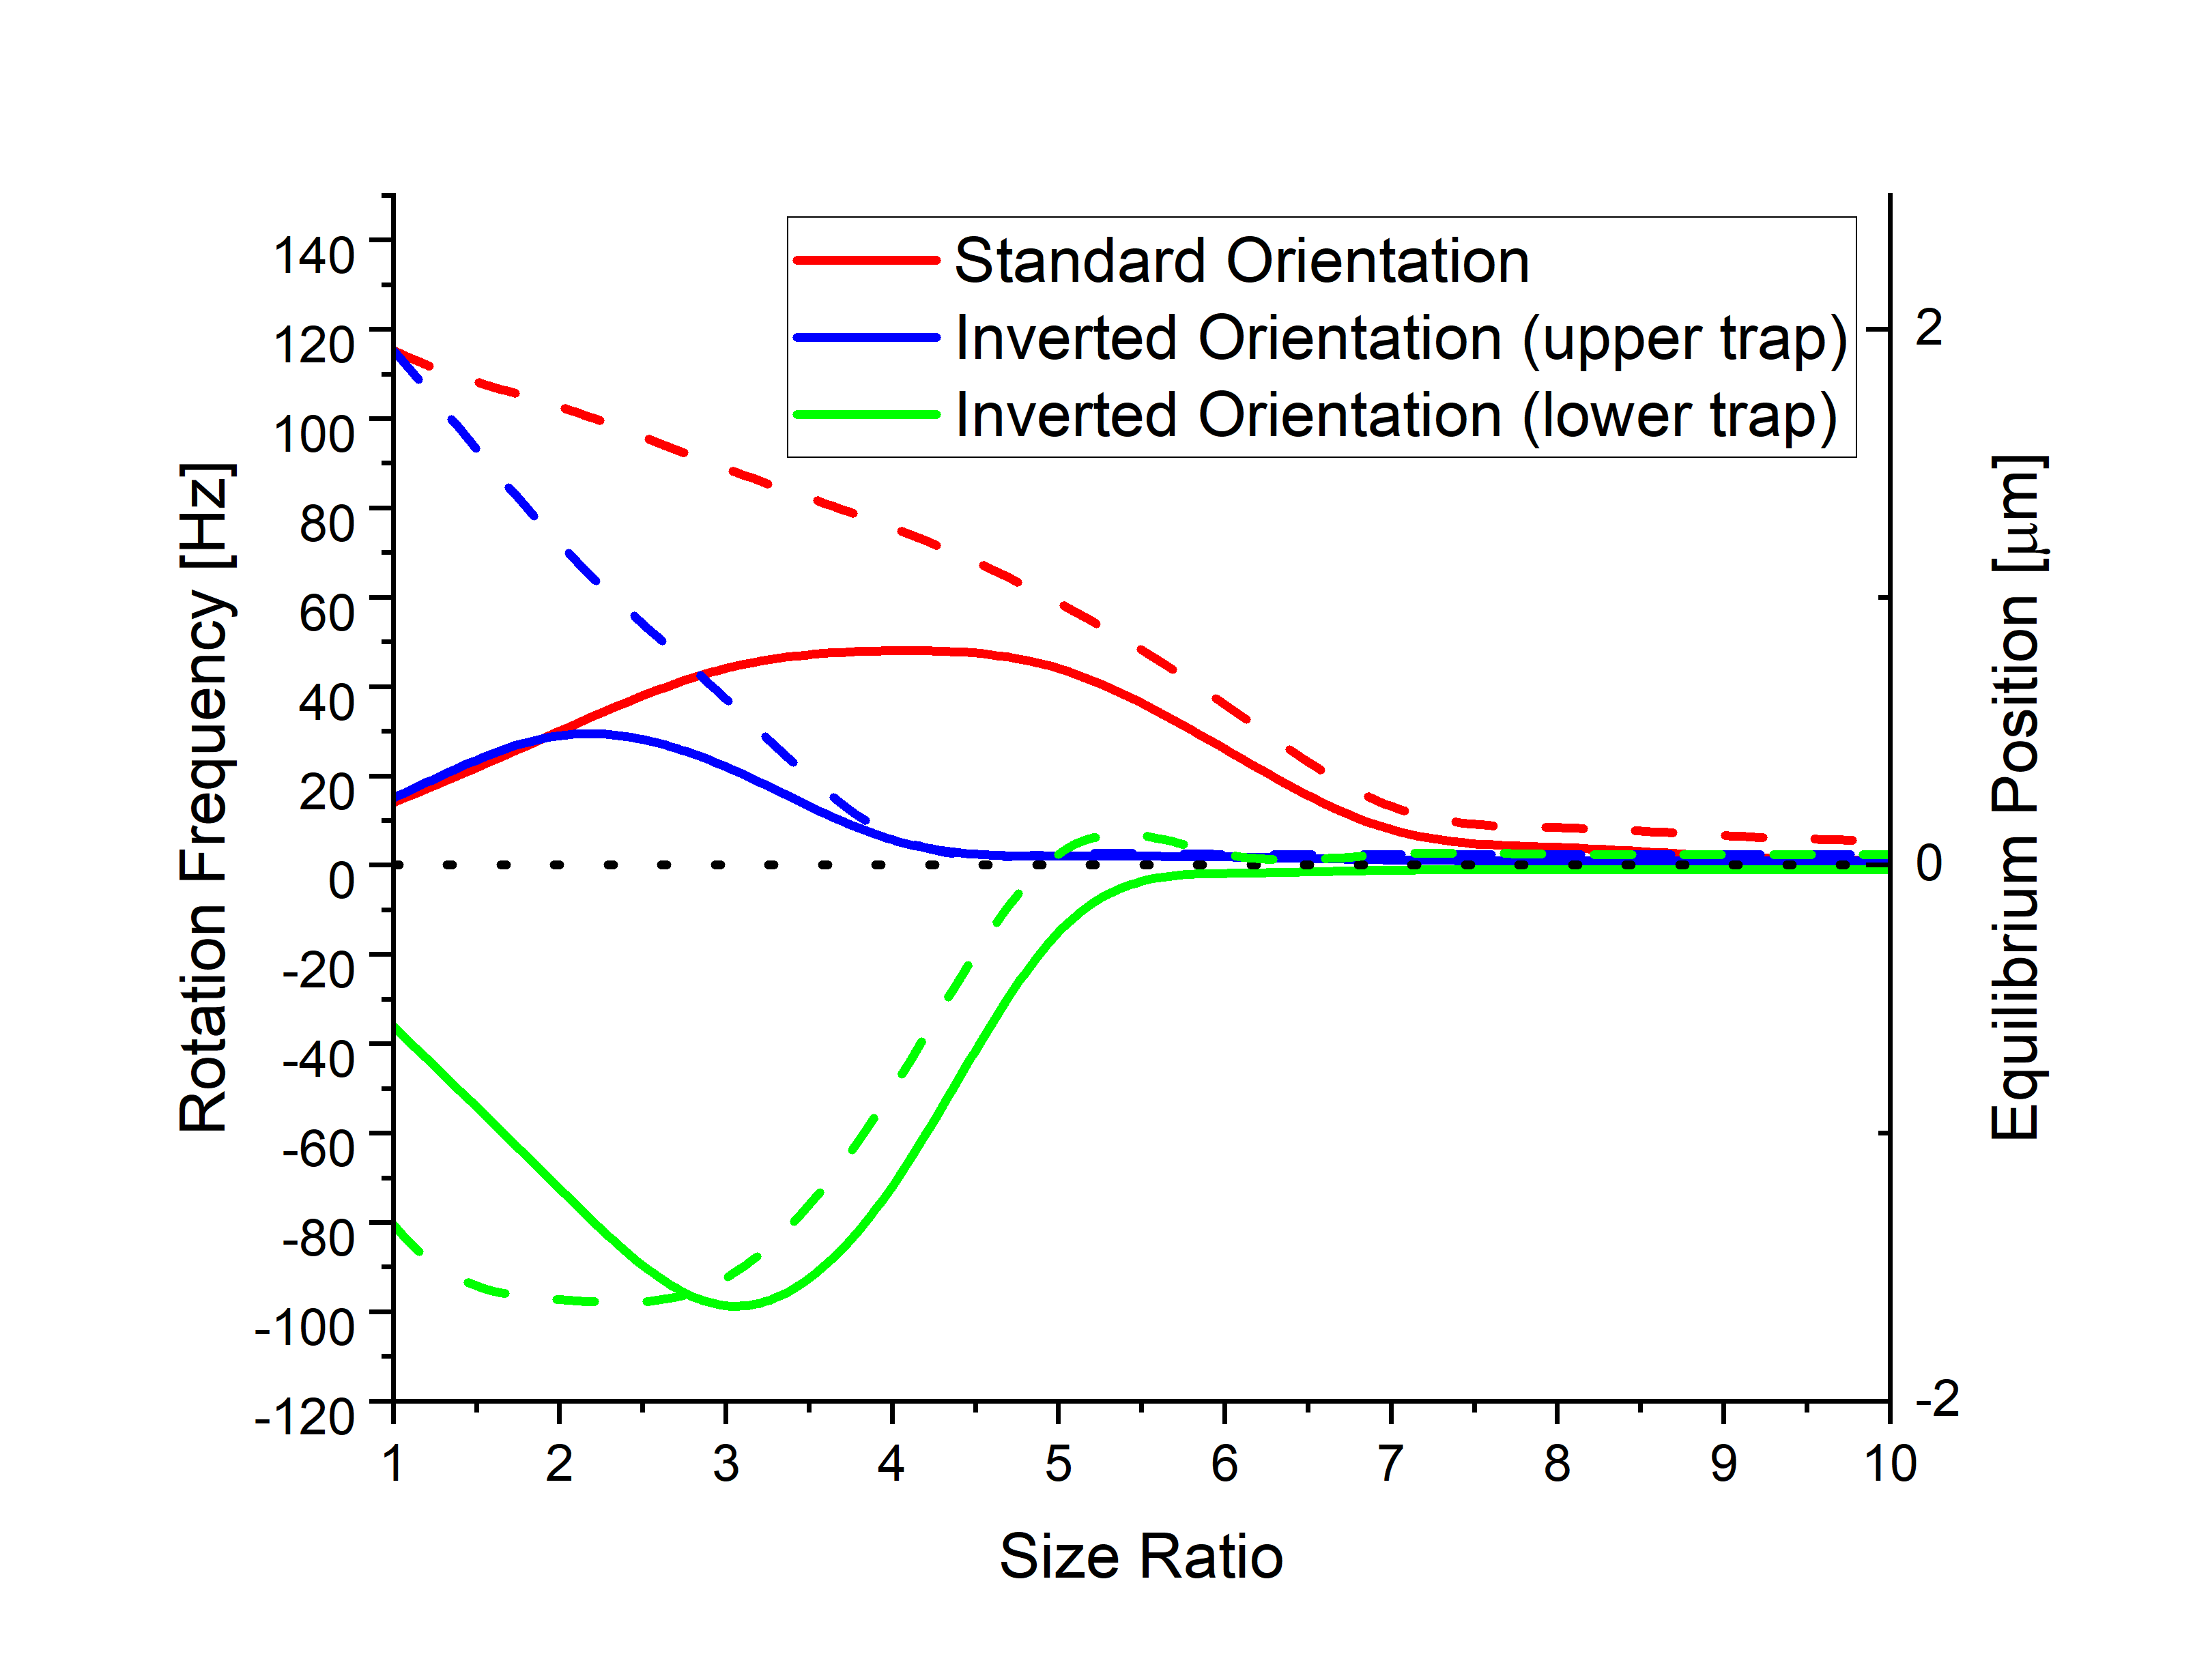
\includegraphics[width=0.65\linewidth]{figs/rotation_rate_vs_size.png}
	\caption{Rotation rate plotted against dimer size ratio for a variety of different simulation scenarios. The red line is for the case where the larger sphere is above the smaller sphere. The blue line is the inverted case, while the initial position is above the focus of the trap. And lastly the green line is again for the inverted case, but when the dimer's initial position is below the focus of the trap.}
\end{figure}

Its difficult to see from the graph, but the rotation rate never truly goes down to zero, reaching a minimum of $~2\ Hz$, which would imply that a second sphere of radius $200\ nm$ is enough to induce rotational motion. These results are somewhat contrary to other work with silica dimers \cite{Ahn2018, Debuysschere2023}; previous experiments have trapped the dimer in an orientation perpendicular to the beam propagation direction. The rotational motion is induced due to the asymmetric geometry creating an unbalanced polarisation susceptibility along its long axis as compared to its short axis; therefore its long axis is aligned with the polarisation vector and can rotate freely\cite{Ahn2018}. This however cannot be the case with our simulations as the dimer rotates about its long axis, meaning there cannot be an asymmetric axis to align with the beam's polarisation vector. Furthermore because most of these experiments operate in the Rayleigh regime orientational effects are not usually considered whereas our own results make it clear that the initial orientation and position of spherical aggregates drastically effects their steady state behaviour.

\newpage

\section{Monitoring Stochastic rotational motion using static light scattering}
Orientational dynamics to an anisotropically scattering shape are difficult to characterise due to the coupling of rotational and translational effects. As shown in the previous chapter the dynamics of even simple dimers are heavily dependent on the particle's position and orientation, this is reflected in literature where several engineering solutions have been devised to decouple translational and orientational motion \textcolor{red}{[ , ]}. While a majority of latter work has been focused on nano-particles (falling into the Rayleigh Regime) and utilising florescence 

\subsection{Coordinate System}
In the case of our probe beam the +z direction points from the surface of the probe directly to the centre of diffusion in our dimer, with the +y direction pointing towards what would be our trapping beam, and the +x direction pointing into the page. The origin of our coordinate system is fixed on the centre of the focus of our trapping beam, meaning as our dimer's centre of diffusion moves the origin is kept constant.
\subsection{Dimer}
The dimer is defined by two spheres, in the trapping frame this would be orientated by $s=[0,0,1]$ however in our scattering set up this is rotated to $s=[-1,0,0]$ as the large sphere is furthest from the trapping beam. We scale the position of each sphere by the factor L:
\begin{align}
	L = \frac{1}{k} = \frac{\lambda}{2\pi}
\end{align}

Where $\lambda$ is the wavelength of light and is given in nanometres, this means every position must be also provided in nanometres.
\subsection{Beam}
Our probe beam is rather simple to define, we firstly say that the probe is a plane wave by setting the Gaussian beam parameter $C_B$ to 0. We also say the beam is un-polarized by defining the Stokes vector as $[1,0,0,0]$. 

\subsection{Detectors and Pixels}

Each detector is placed roughly $2\times 10^5 nm$ from the dimer (can be adjusted later for testing), with the position of the detector being defined by the polar and azimuth angles ($\theta$ \& $\phi$ respectively) such that:
\begin{align}
	[x_{fiber}, y_{fiber}, z_{fiber}] = [rcos(\phi)sin(\theta), rsin(\phi)sin(\theta), rcos(\theta)]
\end{align}
So if you were to place the fibers in the trapping frames x-y plane, in the probe beam frame will only have x and z components. The orientation of the detector is just the -ve of its position and not scaled by the distance term r, the orientation being the vector from the origin of the detector to the center of the dimer. 

Pixels can be thought of as points lying on the surface of the detector, by getting the spherical coordinates of each pixel we can compute the intensity at each point on the detector, allowing us to determine the average intensity on a given detector. The pixels are distributed using a sunflower distribution given by:

Where each point is first scaled to the size of the detector - for now we assume a radius of $2.5 \times 10^4 \ nm$ - and then translated from its position on the surface of the detector to the main coordinate system. Their orientation is treated much in the same as the detector's orientation, being its -ve position and scaled down by the radial distance from the dimer to the pixel, making it a unit vector. From their position we can also grab their spherical coordinates to create a list of points for mstm to evaluate. In order to accurately describe any detector surface we can use a Householder transformation to get the perpendicular circular surface of any vector.

This allows us to define the surface of any detector perpendicular to the origin of our coordinate system, we can freely choose the size and resolution of our fibre's. For every pixel we define the spherical coordinates relative to our origin, this is added to a list of $\theta, \phi$ pairs that are evaluated by MSTM. 

\section{Interpretation of scattering data into orientation estimates}
MSTM is capable of evaluating the scattering characteristics of a given target either in a fixed orientation or using an averaging of the particles orientation. While the latter method is satisfactory for simulation purposes it 

\chapter{Effects of shear flow on the nucleation of crystals}
\section{Shear induced Nucleation}
It has long been known that solution nucleation is influenced by shearing of the fluid, from stirring agents in the container (i.e. propellers) to the container boundary layers, however there has yet to be a clear mechanism by which said shearing effects the nucleation event. Theoretical research into shear induced nucleation suggests that there should be a slight increase in the nucleation rate at low shear rates, reaching a maximum increase in nucleation rate, and then at higher shear rates the nucleation rate begins to drop off. This has been shown theoretically for both simple colloidal \textcolor{red}{[ , ]}  and ice crystal formation\textcolor{red}{[ ]}; however, no experimental work into these systems has been conducted to prove this is the case.  There is some experimental evidence for this phenomena in simple salt and protein solutions - though the authors emphasise that mechanical agitation cannot be ruled out - there has not been a exhaustive study into the shearing effects apart from in glycine solutions. In \textcolor{red}{[ ]} they found that a shear rate of around $3000\ s^{-1}$ was the maximum shear rate that would yield the highest nucleation rate. They tested the theoretical model established in \textcolor{red}{[ ]} which modifies the CNT to account for the effects of a nucleus undergoing shearing; they accounted for the fact that a nucleus' growth is undergoing competition between flow-mediated molecular transport and the strain applied by the flow field which inhibits the growth of the nucleus. There central conclusion (from both the theoretical and experimental results) is that there is an optimal shear rate in which the nucleation rate is maximised. However, a question that arises from this result, if there is a optimal shear rate in which molecular transport is maximised and strain is minimised, then surely there should also be a shear rate in which the molecular transport and strain are equal - allowing one to suspend a nucleus at a constant radius. In this scenario, the molecular transport would prevent the nucleus from dissolving, but the strain would prevent the nucleus from growing. This however would require one to be able to apply a continuous shear rate to a targeted nucleus with high precision, there is also no model for an individual nucleus undergoing growth. 

Optical tweezing has often been used for micro-rheology, by computing the exact forces being exerted on the trapped sphere, one can determine the fluid viscosity of the local surrounding medium. Typically one would use a birefringent particle (i.e. vaterite) and rotating it within the fluid, the maximum rotation rate being a product of the fluid drag resisting the torque of the trapping beam. Likewise, one can use a galvanometric mirror to probe the drag force of the fluid, by understanding the trap strength (calibrating using a low frequency signal) one can compute the force required to escape the trap and likewise determine the drag force applied by a moving sphere. Likewise, one can perform the inverse experiment, by applying a known shear rate one can see how the fluid responds to the fluid shear; this is what we attempt with the galvano-mirror, how does a supersaturated solution respond to a localised fluid field? This requires that we both know the fluid velocity, and the shear rate applied by our probe particle. Furthermore, we also require an understanding of how the fluid is effected by the beam, both the temperature rise and the corresponding change to the fluid viscosity. 

Understanding the fluid velocity around our trapped object is determined mostly by the Reynold's number of our system, for a sphere submersed in a moving fluid of velocity $U$ this is given by:
\begin{align}
	Re = \frac{\rho UD}{\mu}
\end{align}
Where $D$ is the sphere's diameter, and $\rho$ and $\mu$ are the fluid's density and viscosity respectively. In our case we do not have a fluid moving around a sphere but a sphere moving through the fluid at some velocity $U$, assuming a no-slip boundary condition we can model the fluid velocity profile based on the velocity of the particle. There are two possible avenues for generating shear flow with a trapped particle; rotation of birefringent particles, and fluid flow induced by particle motion. 

Rotating birefringent particles are by far the most common method for generating and measuring fluid flow in a solution. To see if we can even achieve the theoretical maximum shear rate, vaterite spheres were synthesised (see Sec.\ref{sec:vaterite}) submerged in water and trapped with the 1064 nm laser at set to 450 mW. The rotation frequency was determined using the QPD, and the particle sizes were computed by image analysis. With the particle size and rotation frequency, the tangential rotation speed is calculated via:

\begin{align}
	\label{eq:birefringent_speed}
	u(r) = \frac{\pi}{4}\frac{d^3}{r^2}\omega
\end{align}

Where $d$ is the particle diameter, $\omega$ is the rotation frequency reported by the QPD, and $r$ is the distance from the particle's centre. Using Eq.\ref{eq:birefringent_speed} we computed the fluid flow radiating outward from the centre of the sphere. The shear rate can then be computed as the partial derivative fluid flow (assuming shearing is generated purely by the flow field):

\begin{align}
	\label{eq:birefringent_shear}
	\dot{\gamma}(r)=\left|\frac{\delta u(r)}{\delta r} \right|= \frac{\pi}{2}\frac{d^3}{r^3}\omega
\end{align}

\begin{figure}[h]
	\label{fig:vaterite_shear}
	\begin{subfigure}{0.5\linewidth}
		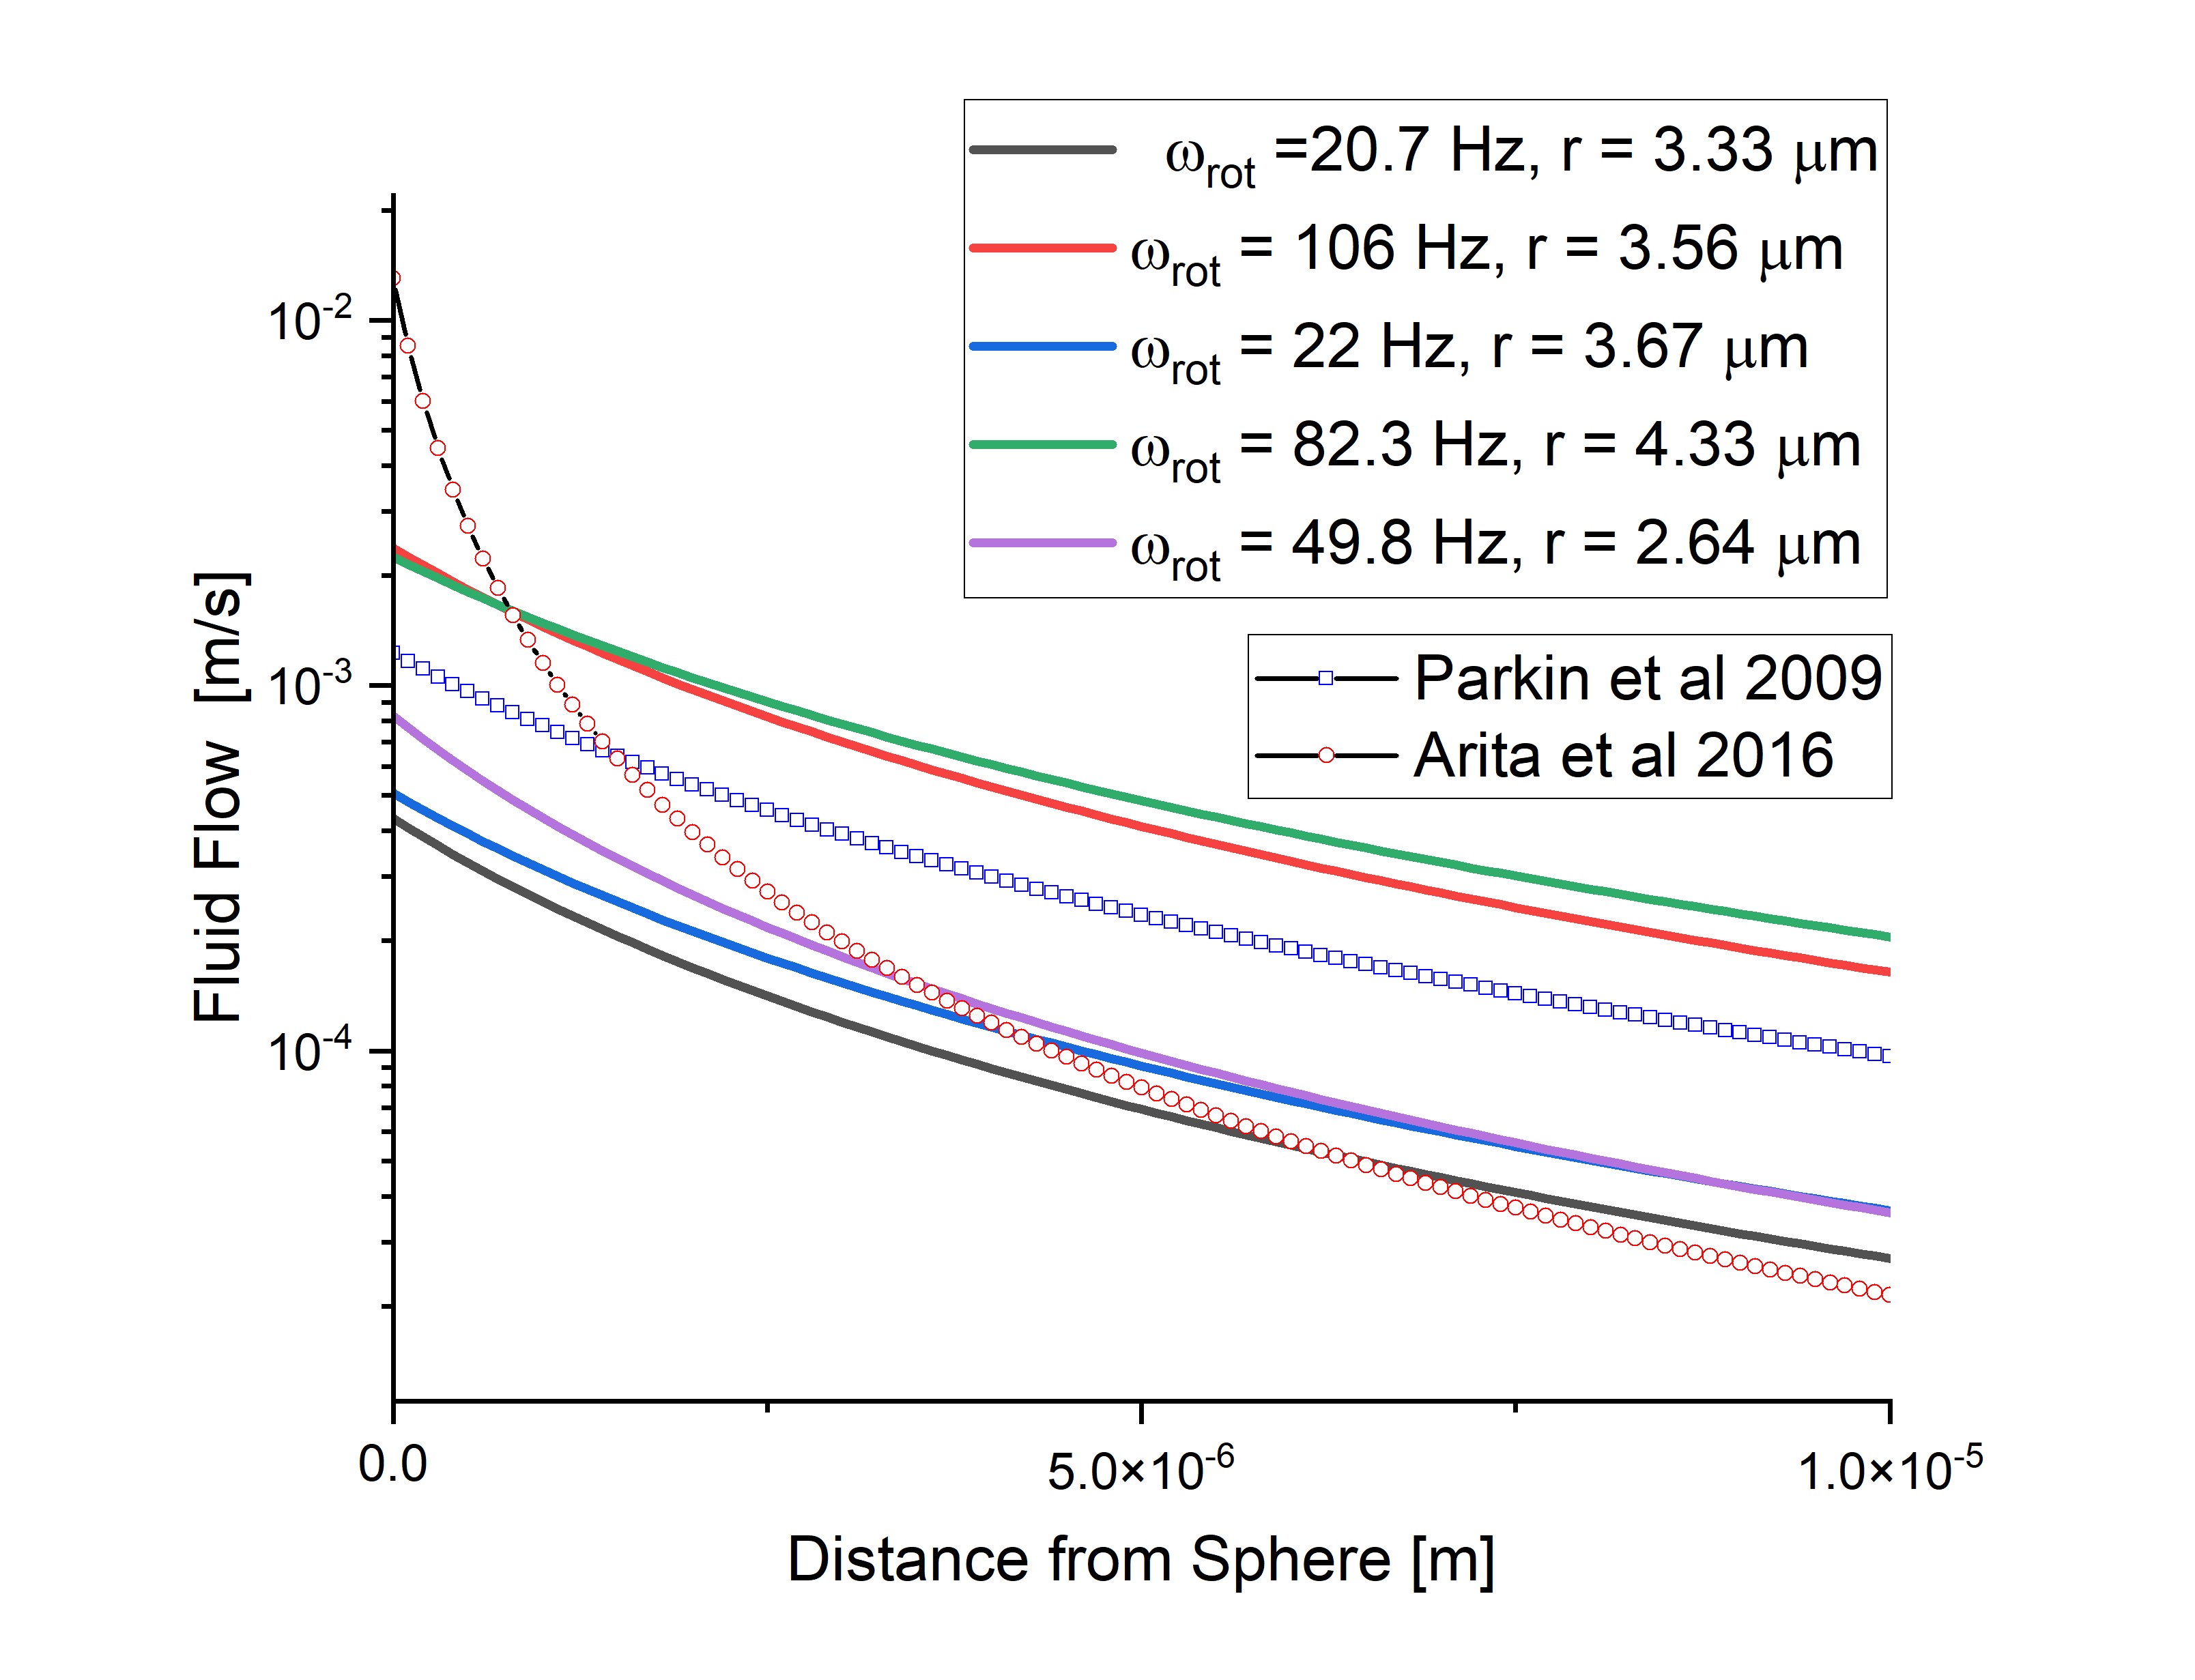
\includegraphics[width=\linewidth]{figs/vaterite_fluid_flow.png}
		\subcaption{}
	\end{subfigure}
	\begin{subfigure}{0.5\linewidth}
		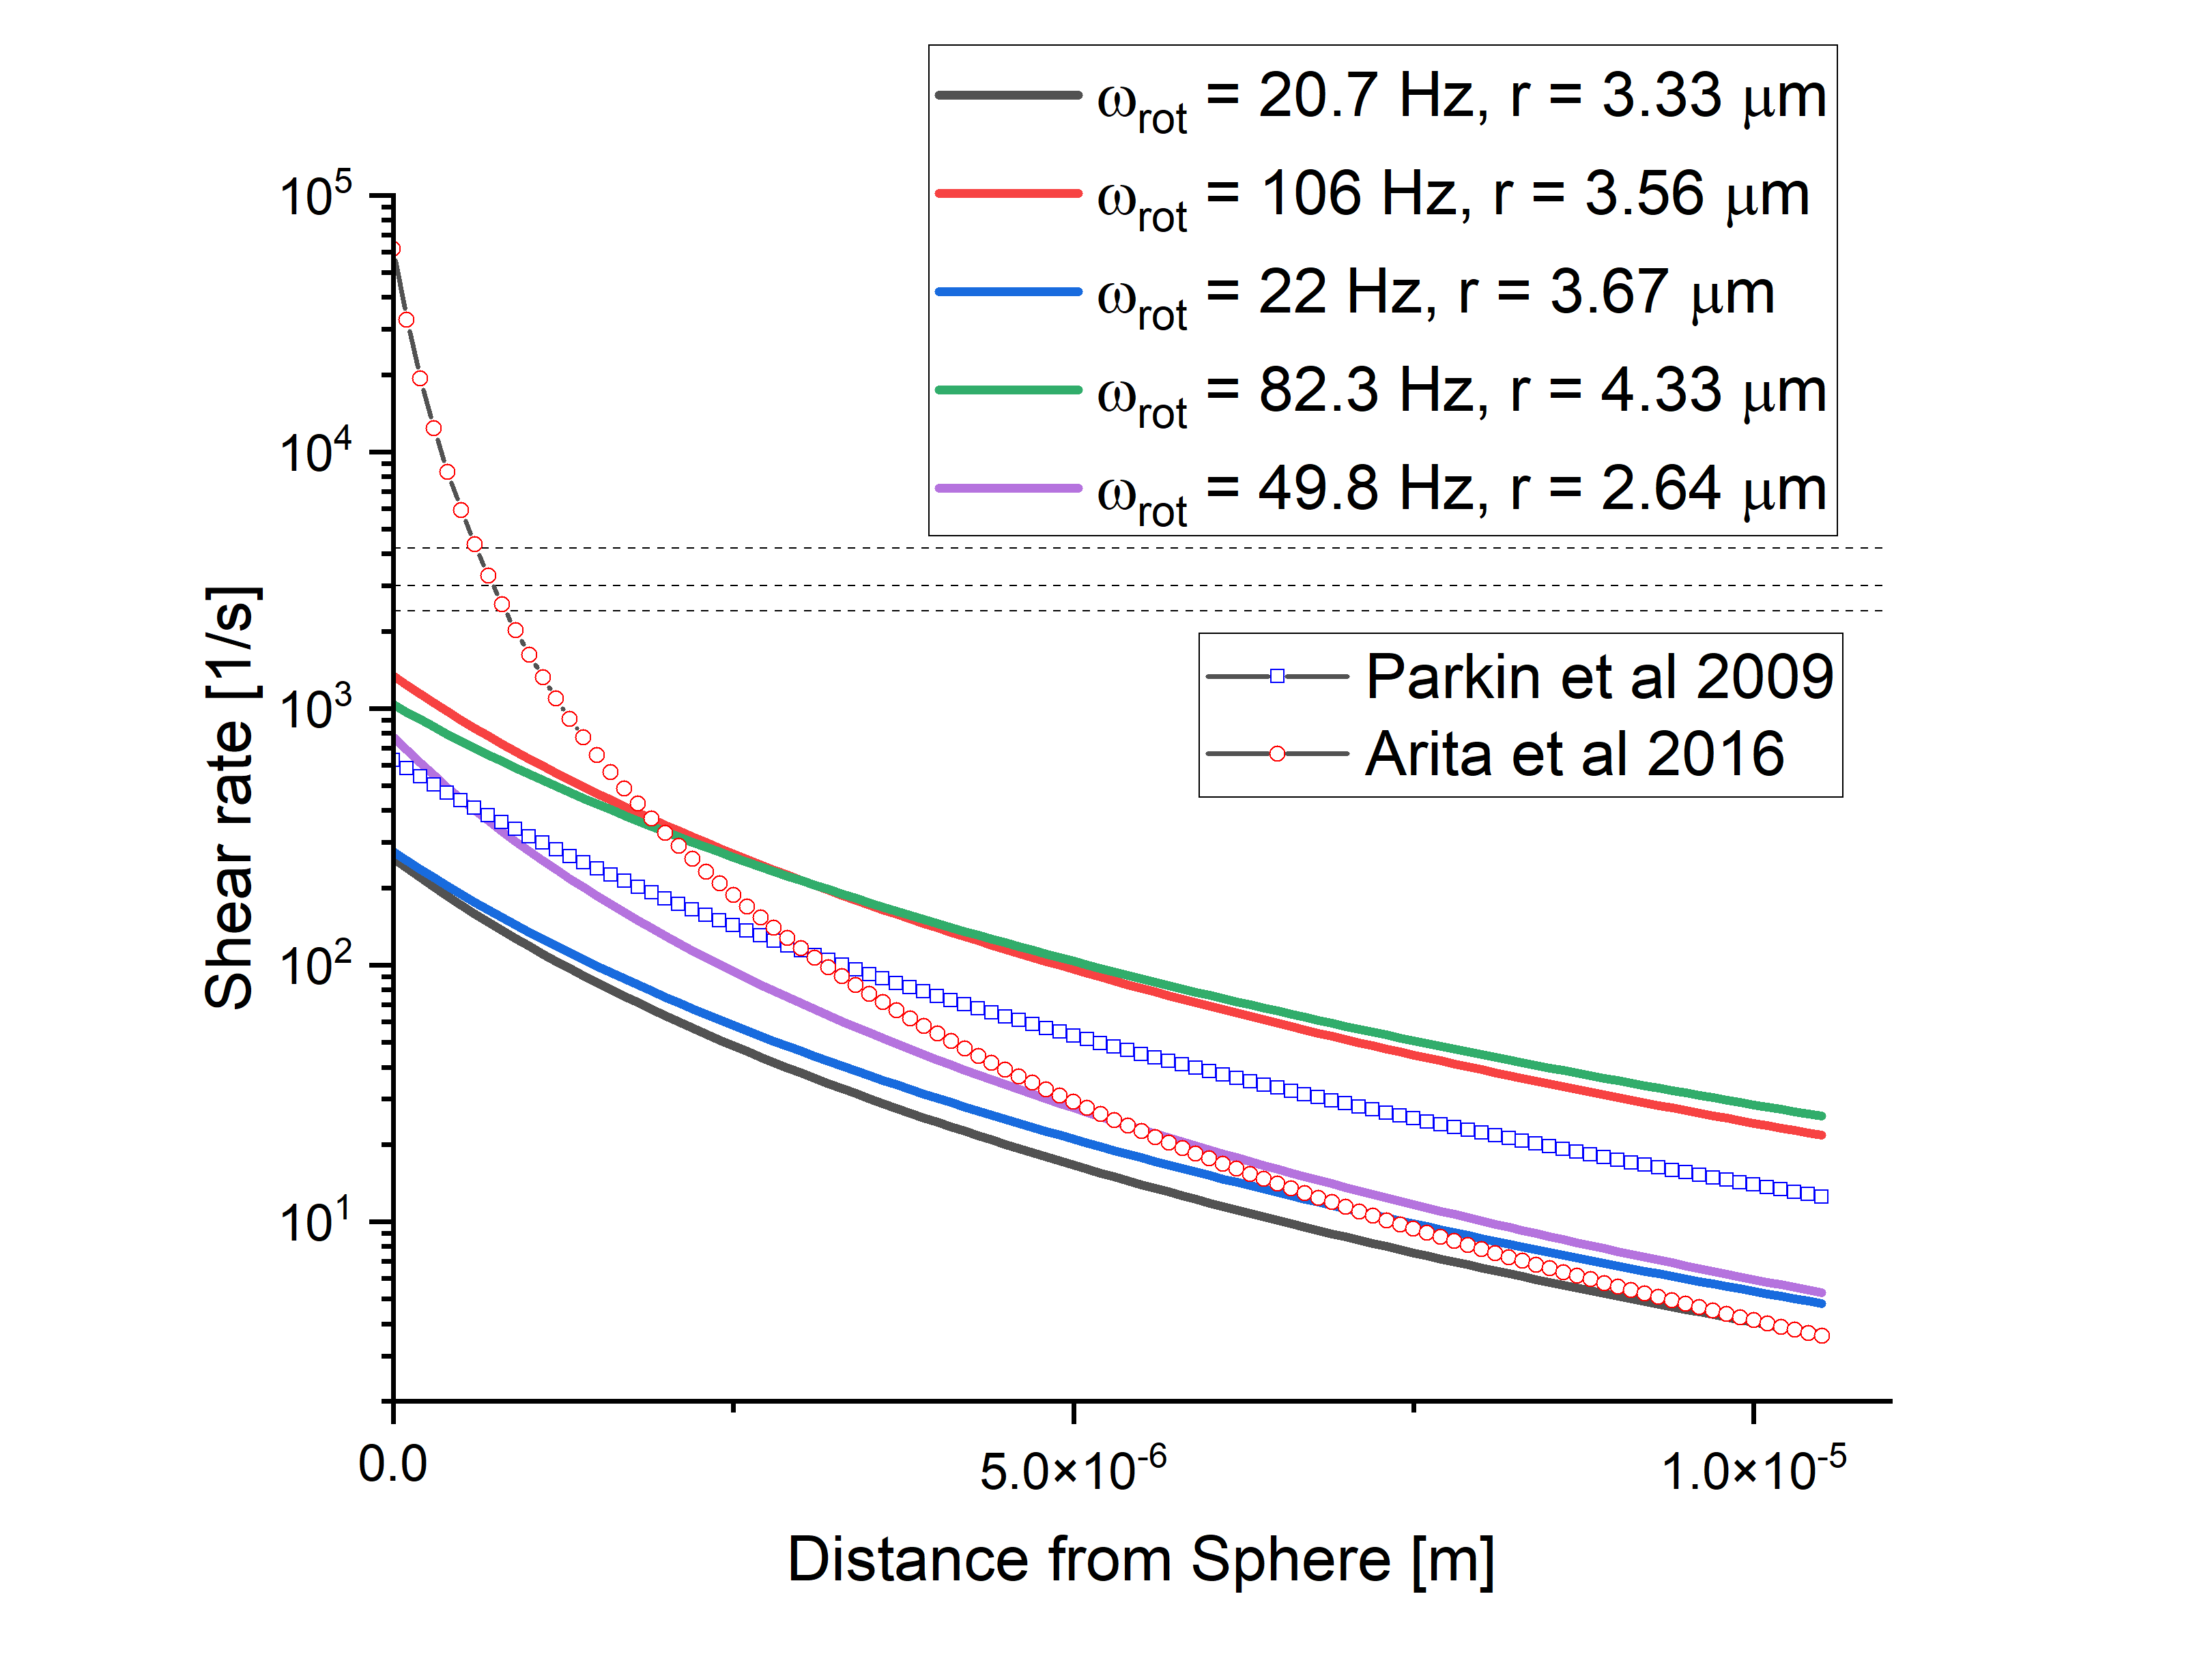
\includegraphics[width=\linewidth]{figs/vaterite_shear_rate.png}
		\subcaption{}
	\end{subfigure}
	\caption{(a) Fluid flow radiating out from the surface of a rotating vaterite sphere. (b) Shear rates computed using Eq.\ref{eq:birefringent_shear}, optimal shear rate is of $3000 s^{-1}$ is indicated by the dotted line. Vaterite radii and rotation frequencies are shown, the laser power was kept constant at 450 mW. Reported rotation rates, and their corresponding fluid flow and shear rates, for vaterite are also plotted alongside lab results.}
\end{figure}

From Fig.\ref{fig:vaterite_shear} it's clear that 

Using a galvano mirror can A particle's motion can be precisely controlled For a simple circular path one can estimate the sphere's speed by the radius of its path and the frequency of its orbit $U = R\omega$; however for a more complex path, such as an elliptical orbit the curve needs to be parametrised. One can describe the position parameter of an ellipse as such:

\begin{align}
	r(u) = \left[acos(2\pi u),bsin(2\pi u), 0 \right]
\end{align}

where a and b are the different characteristic radii of an ellipse, if we assume that u describes time from some initial point we can say $u=t\omega$ where omega is the frequency of orbit. Subbing this in and then taking the partial derivative of position gives:

\begin{align}
	v(t) = \frac{dr(t)}{dt} = \left[-2\pi a\omega \ sin(2\pi t\omega),\ 2\pi b\omega \ cos(2\pi t\omega),0 \right]
\end{align}

In order to compute U we simply take the magnitude of our velocity. For low velocities the fluid flow around the entire sphere can be computed based on the sphere's velocity.

\begin{align}
	u_r(r)=-v(t)cos(\theta)\left(1-\frac{3R}{2r}+\frac{R^3}{2r^3}\right)
\end{align}

Where $\theta$ is the angle from the direction of movement to the point you wish to measure, and $r$ is the radial distance to that point. Again taking the partial derivative we can get the shear rate for a particle moving through the fluid:

\begin{align}
	\dot{\gamma}(r) = \left| \frac{\delta u_r(r)}{\delta r}\right| = v(t)cos(\theta)\left(\frac{3R}{r^2} -\frac{2R^3}{r^4} \right)
\end{align}

Silica beads ($r=1,57 \mu m$) were trapped and moved along an elliptical path

\chapter{Closing Remarks}



%%%%%%%%%%%%%%%%%%%%%%%%%%%%%%%%%%%%%%%%%%%%%%%%%%%%%%%%%%%%%%
\appendix
\chapter{Stuff That Didn't Fit Anywhere Else}
%%%%%%%%%%%%%%%%%%%%%%%%%%%%%%%%%%%%%%%%%%%%%%%%%%%%%%%%%%%%%%

%%%%%%%%%%%%%%%%%%%%%%%%%%%%%%%%%%%%%%%%%%%%%%%%%%%%%%%%%%%%%%
\addcontentsline{toc}{chapter}{Bibliography}
\bibliographystyle{ieeetran}
\bibliography{thesis_bib}

\end{document}